\documentclass[../Matt_Gebert_Honours_Thesis.tex]{subfiles}

\begin{document}
% The results to here will be compared alongside data after stamping the same devices with thin oxides in  \cref{chap:thinoxidegraphene}.

	In this chapter, I explore various liquid metal stamping techniques\cite{zavabeti_liquid_2017} that were further developed through my work to transfer oxides on a graphene device. Progress towards successful oxide transfer was achieved by using many dummy devices consisting of gold pads but no device.
	
	During this time I worked closely with Kourosh Kalantar-zadeh's group at RMIT (Royal Melbourne institute of technology), in particular Ali Zavabeti, Torben Daeneke, Nitu Syed, Hareem Khan and Paul Atkin in developing this work.

	\section{Printing}\label{sec:printing}
		The traditional technique of mechanical exfoliation is at the core creating many new materials in current research. This is also the case with the liquid metal stamping technique. In this section, I will discuss \aluminimumoxide{}, \tinoxide{} and \bismuthoxide{}, all of which are synthesised by `stamping' onto liquid metal droplets. 
		
	\subsection{Al$_2$O$_3$}
		Aluminium oxide was the first oxide Ali and I investigated for use in our devices. This was for the reason that generally \aluminimumoxide{} is very easy to make by grinding up aluminium wire. I have already detailed the bare process in \cref{sec:oxidestamp_chap2}. An example of the droplets created using the mortar and pestle is seen in \cref{fig:al_synthesis}, and the touching process.		
		\begin{figure}[H]
			\centering
			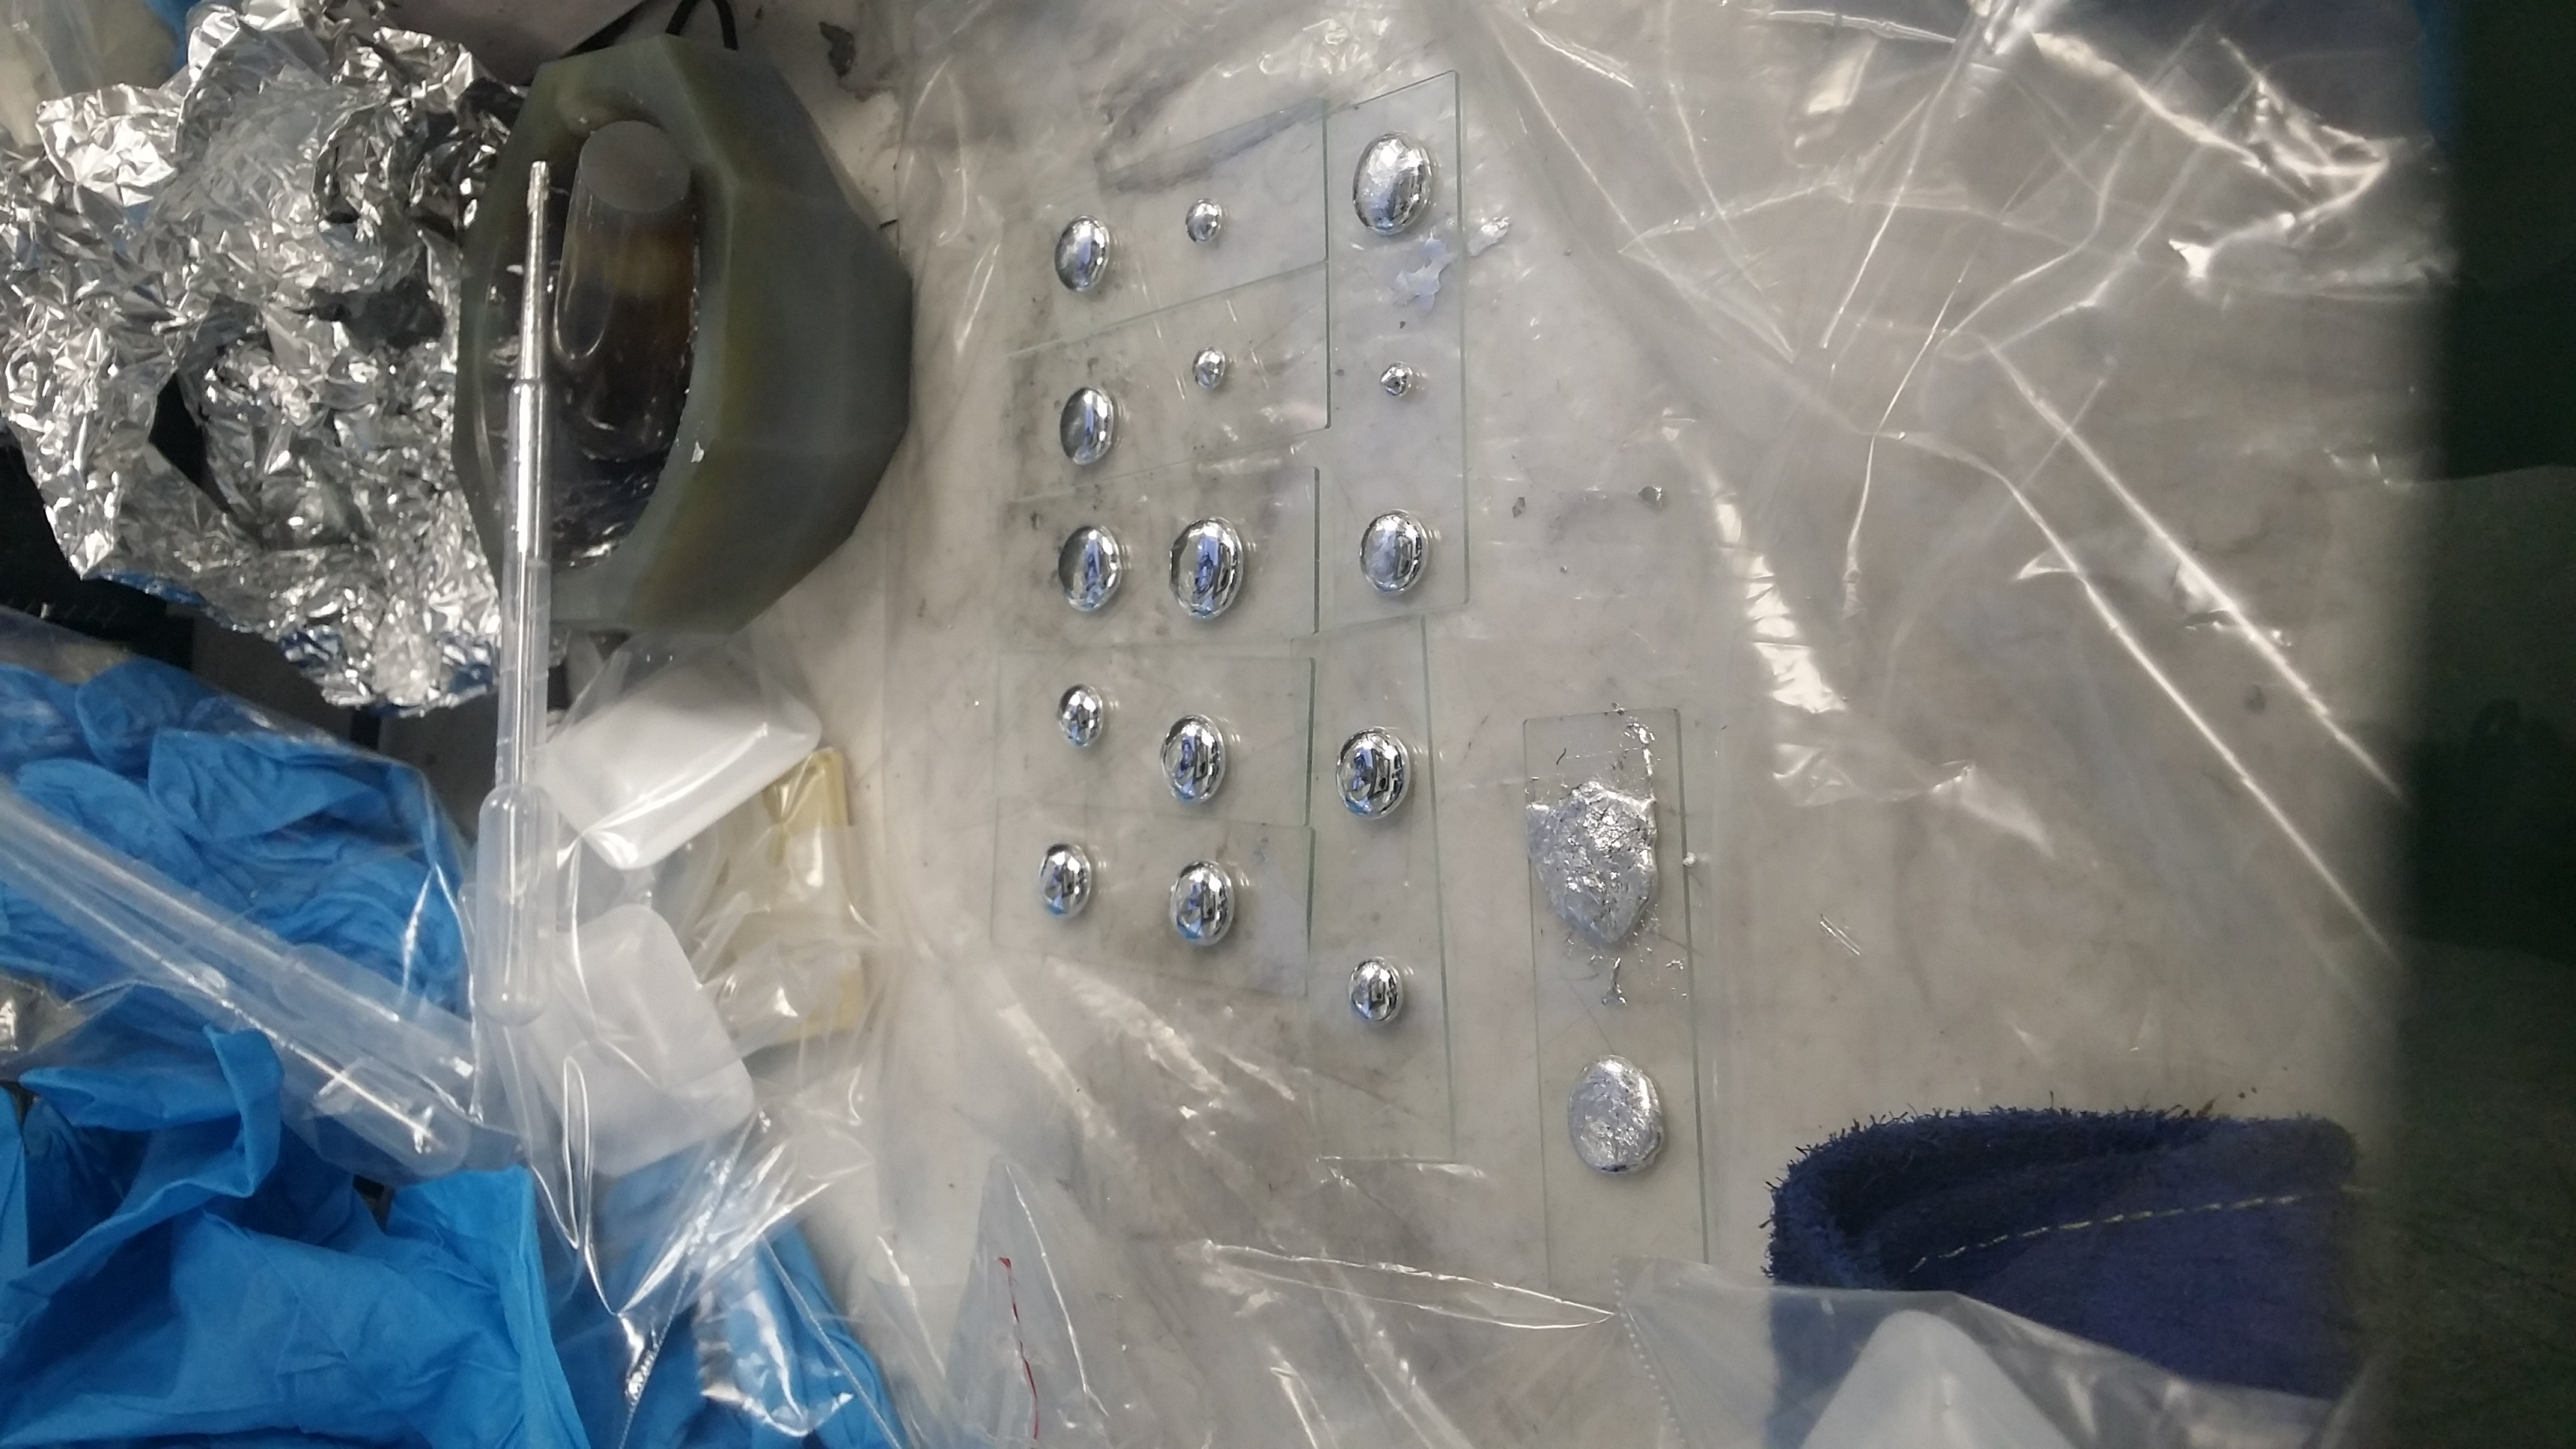
\includegraphics[width=0.3\textwidth,angle=270]{chap5/al2o3/setup}
			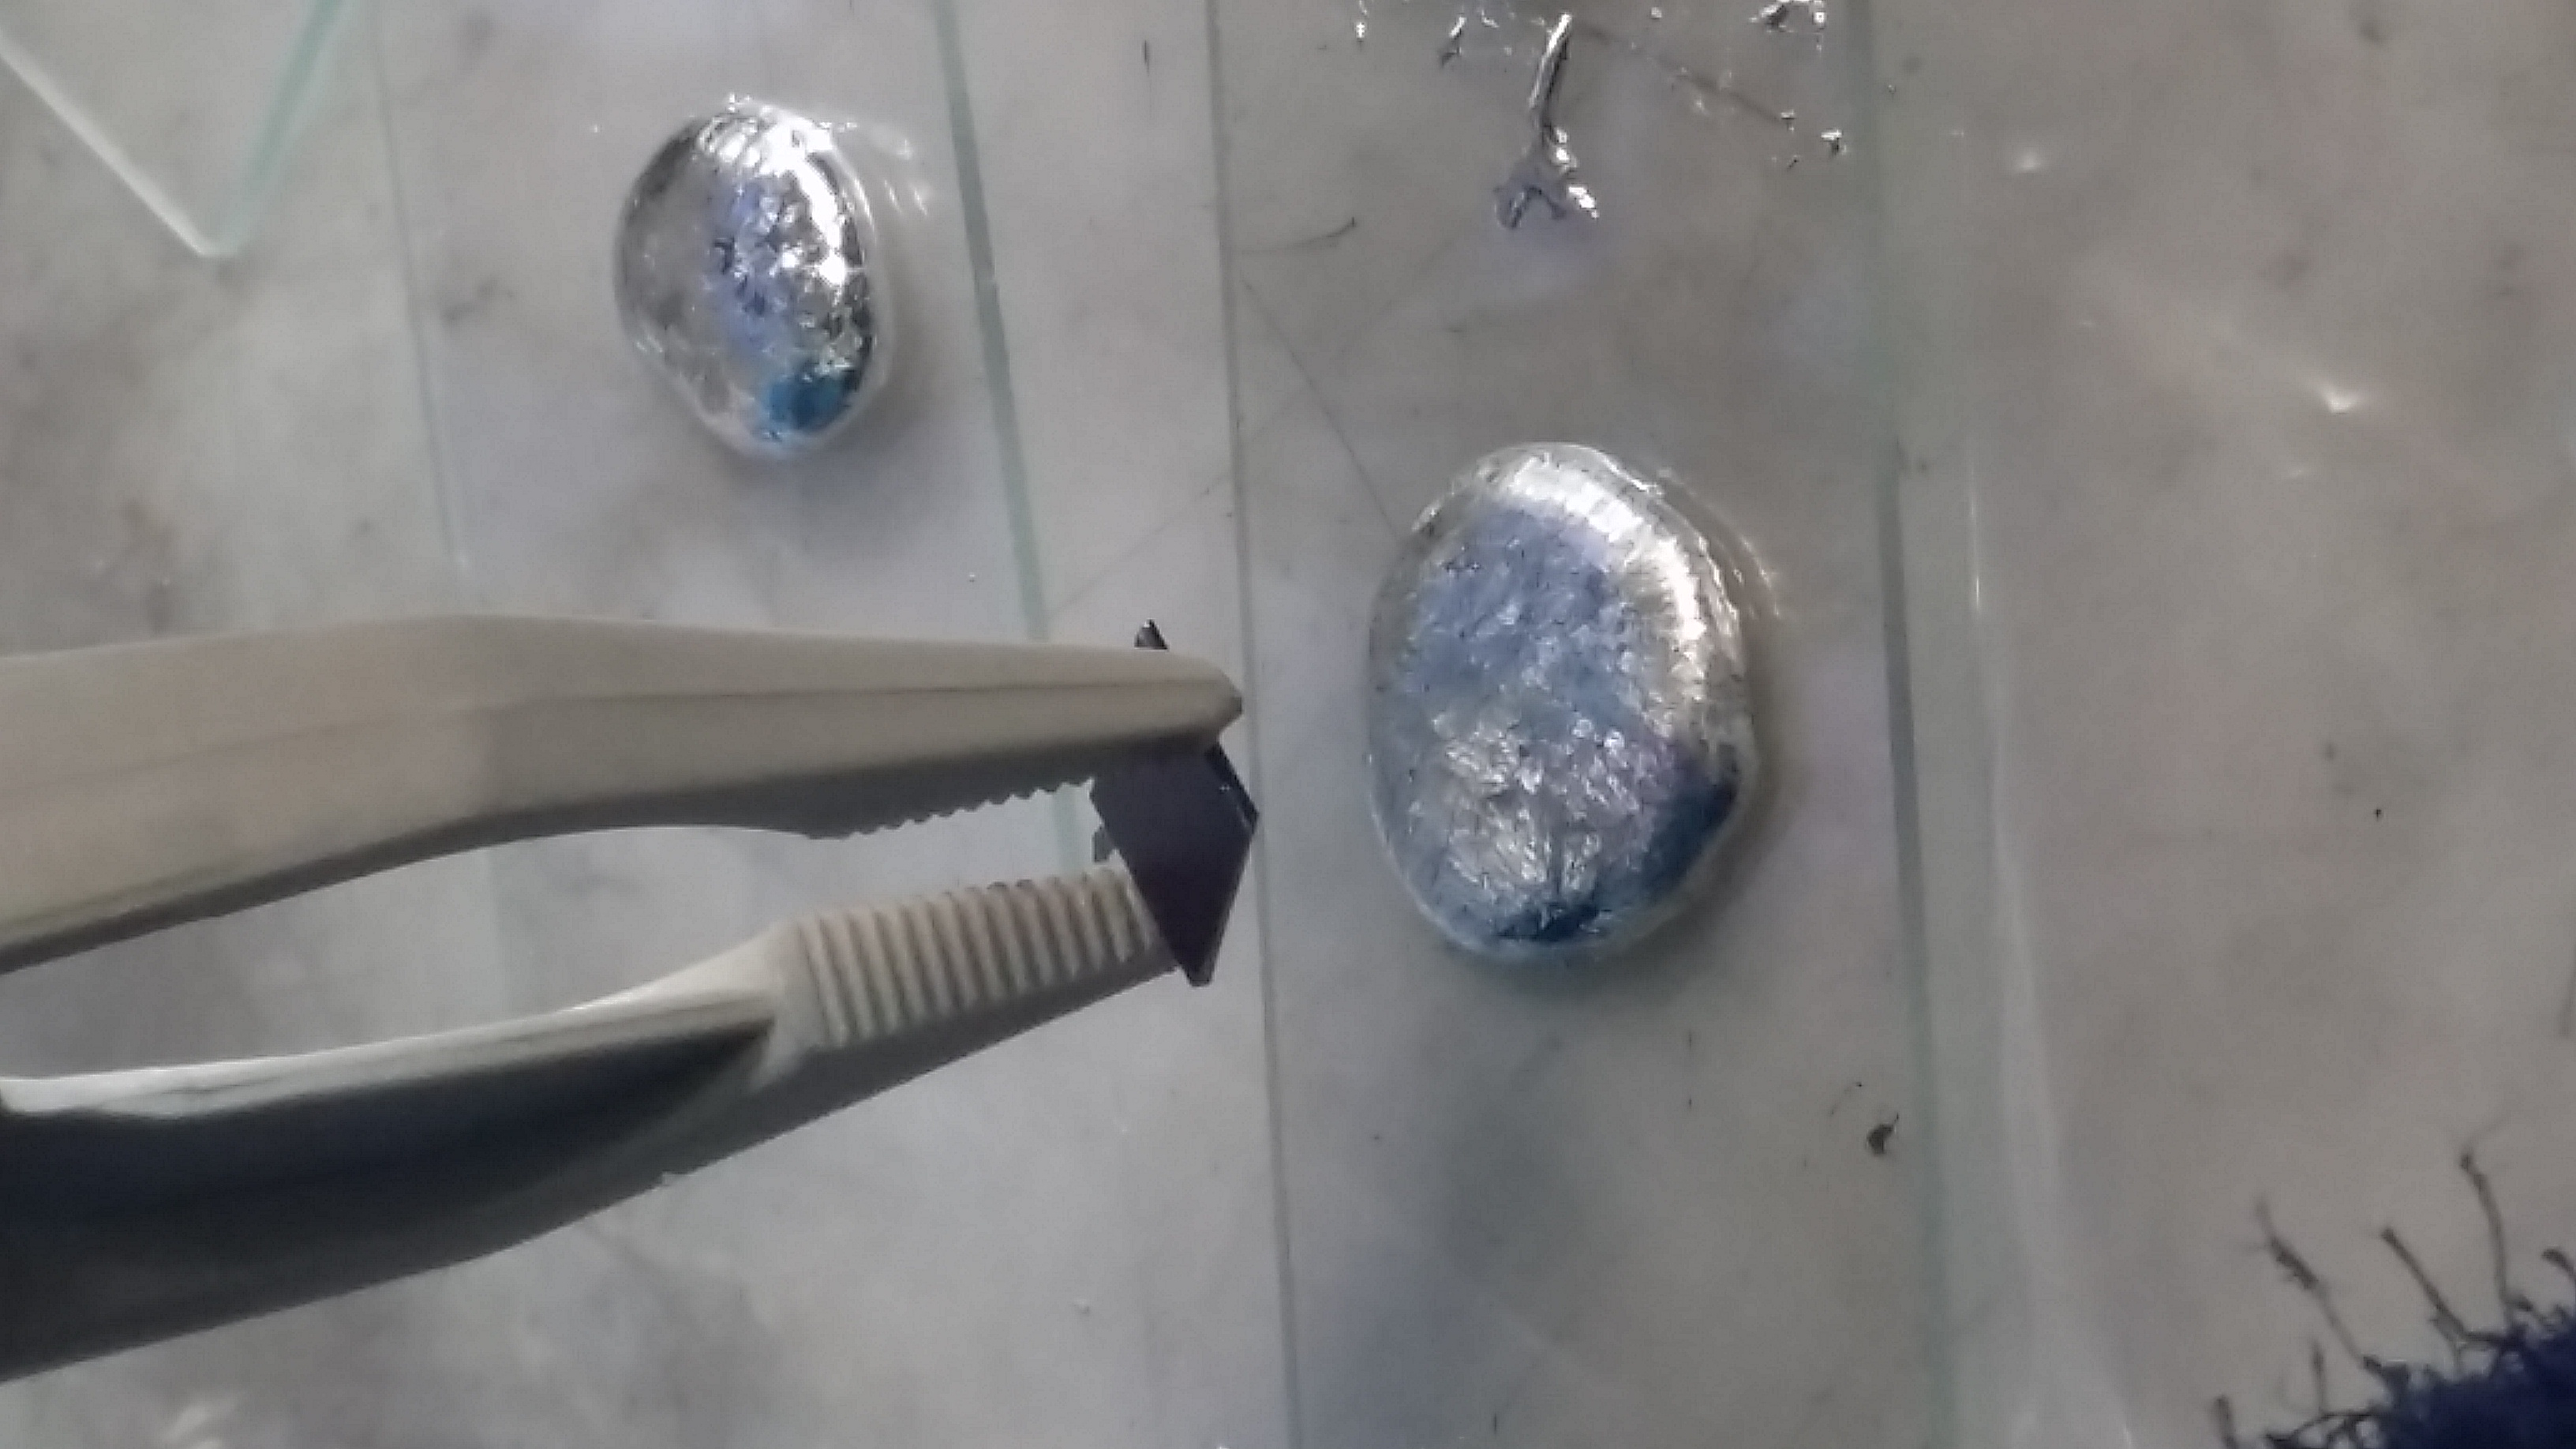
\includegraphics[width=0.3\textwidth,angle=270]{chap5/al2o3/stamp}
			\caption[\aluminimumoxide{} synthesis process]{Synthesis process for stamping \aluminimumoxide{} }\label{fig:al_synthesis}
		\end{figure}
		We tested over 30 samples on droplets, varying radii and exposure time to air (to let the oxide form on the surface). Unfortunately very little material transferred in any of these tests, with only one clean deposition as shown in \cref{fig:al2o3_1}. 
		\begin{figure}[H]
			\begin{subfigure}[t]{0.5\textwidth}
				\centering
				\includegraphics[width=0.85\textwidth,angle=0]{chap5/al2o3/transfer1}
				\caption{\aluminimumoxide{} on \silicondioxide{} (unknown thickness).}\label{fig:al2o3_1}
			\end{subfigure}
			\begin{subfigure}[t]{0.5\textwidth}
				\centering
				\includegraphics[width=0.85\textwidth,angle=0]{chap5/al2o3/transfer2}
				\caption{Non uniform oxide deposition, but some thin areas}\label{fig:al2o3_2}
			\end{subfigure}
			\begin{subfigure}[t]{0.5\textwidth}
				\centering
				\includegraphics[width=0.85\textwidth,angle=0]{chap5/al2o3/transfer3}
				\caption{Metal residue left after an unsuccessful transfer}\label{fig:al2o3_3}
			\end{subfigure}
			\begin{subfigure}[t]{0.5\textwidth}
				\centering
				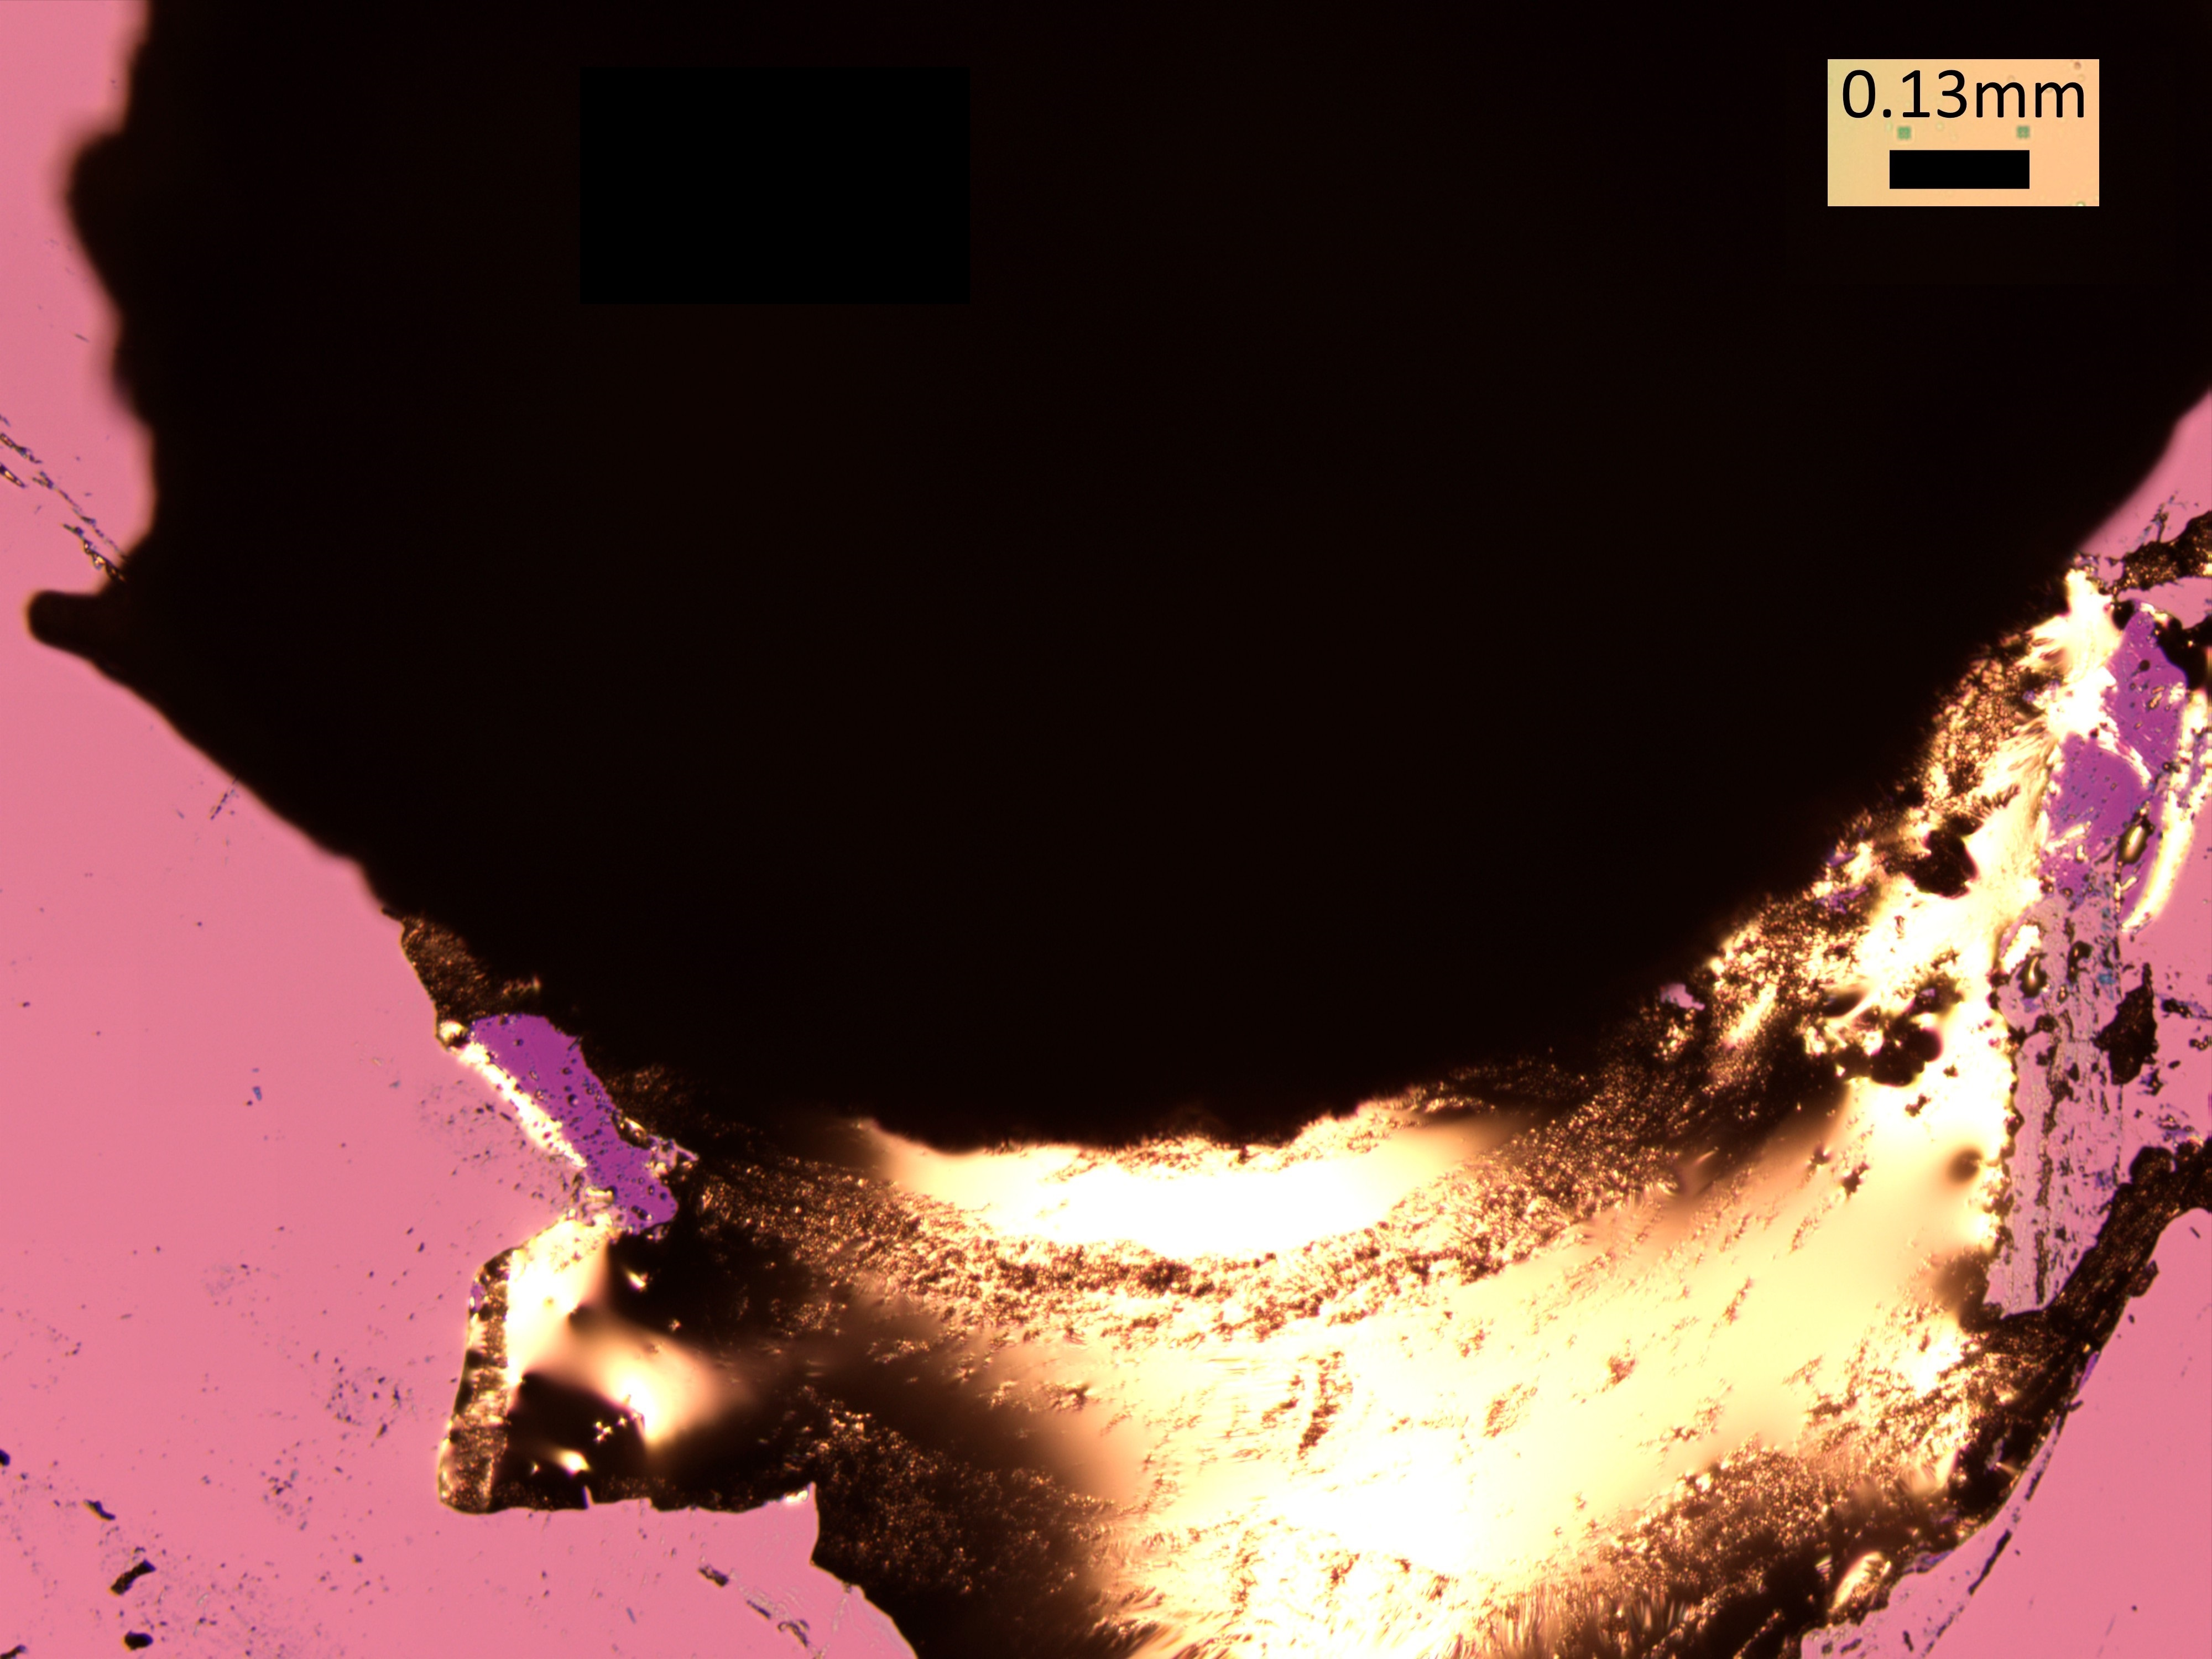
\includegraphics[width=0.85\textwidth,angle=0]{chap5/al2o3/transfer4}
				\caption{Metal remaining, with traces of thick (gallium) oxide}\label{fig:al2o3_4}
			\end{subfigure}
		\caption[\aluminimumoxide{} stamped on \silicondioxide{}]{Deposition of \aluminimumoxide{} onto \silicondioxide{}. Scale bar: 0.13mm}\label{fig:transfer_al_on_si}
		\end{figure}
		More commonly than not though, the liquid metal begun interacting with gold pads and adhering through any oxide layer, or no oxide was deposited (\cref{fig:transfer_al_on_au&si})
		\begin{figure}[H]
			\begin{subfigure}[t]{0.5\textwidth}
				\centering
				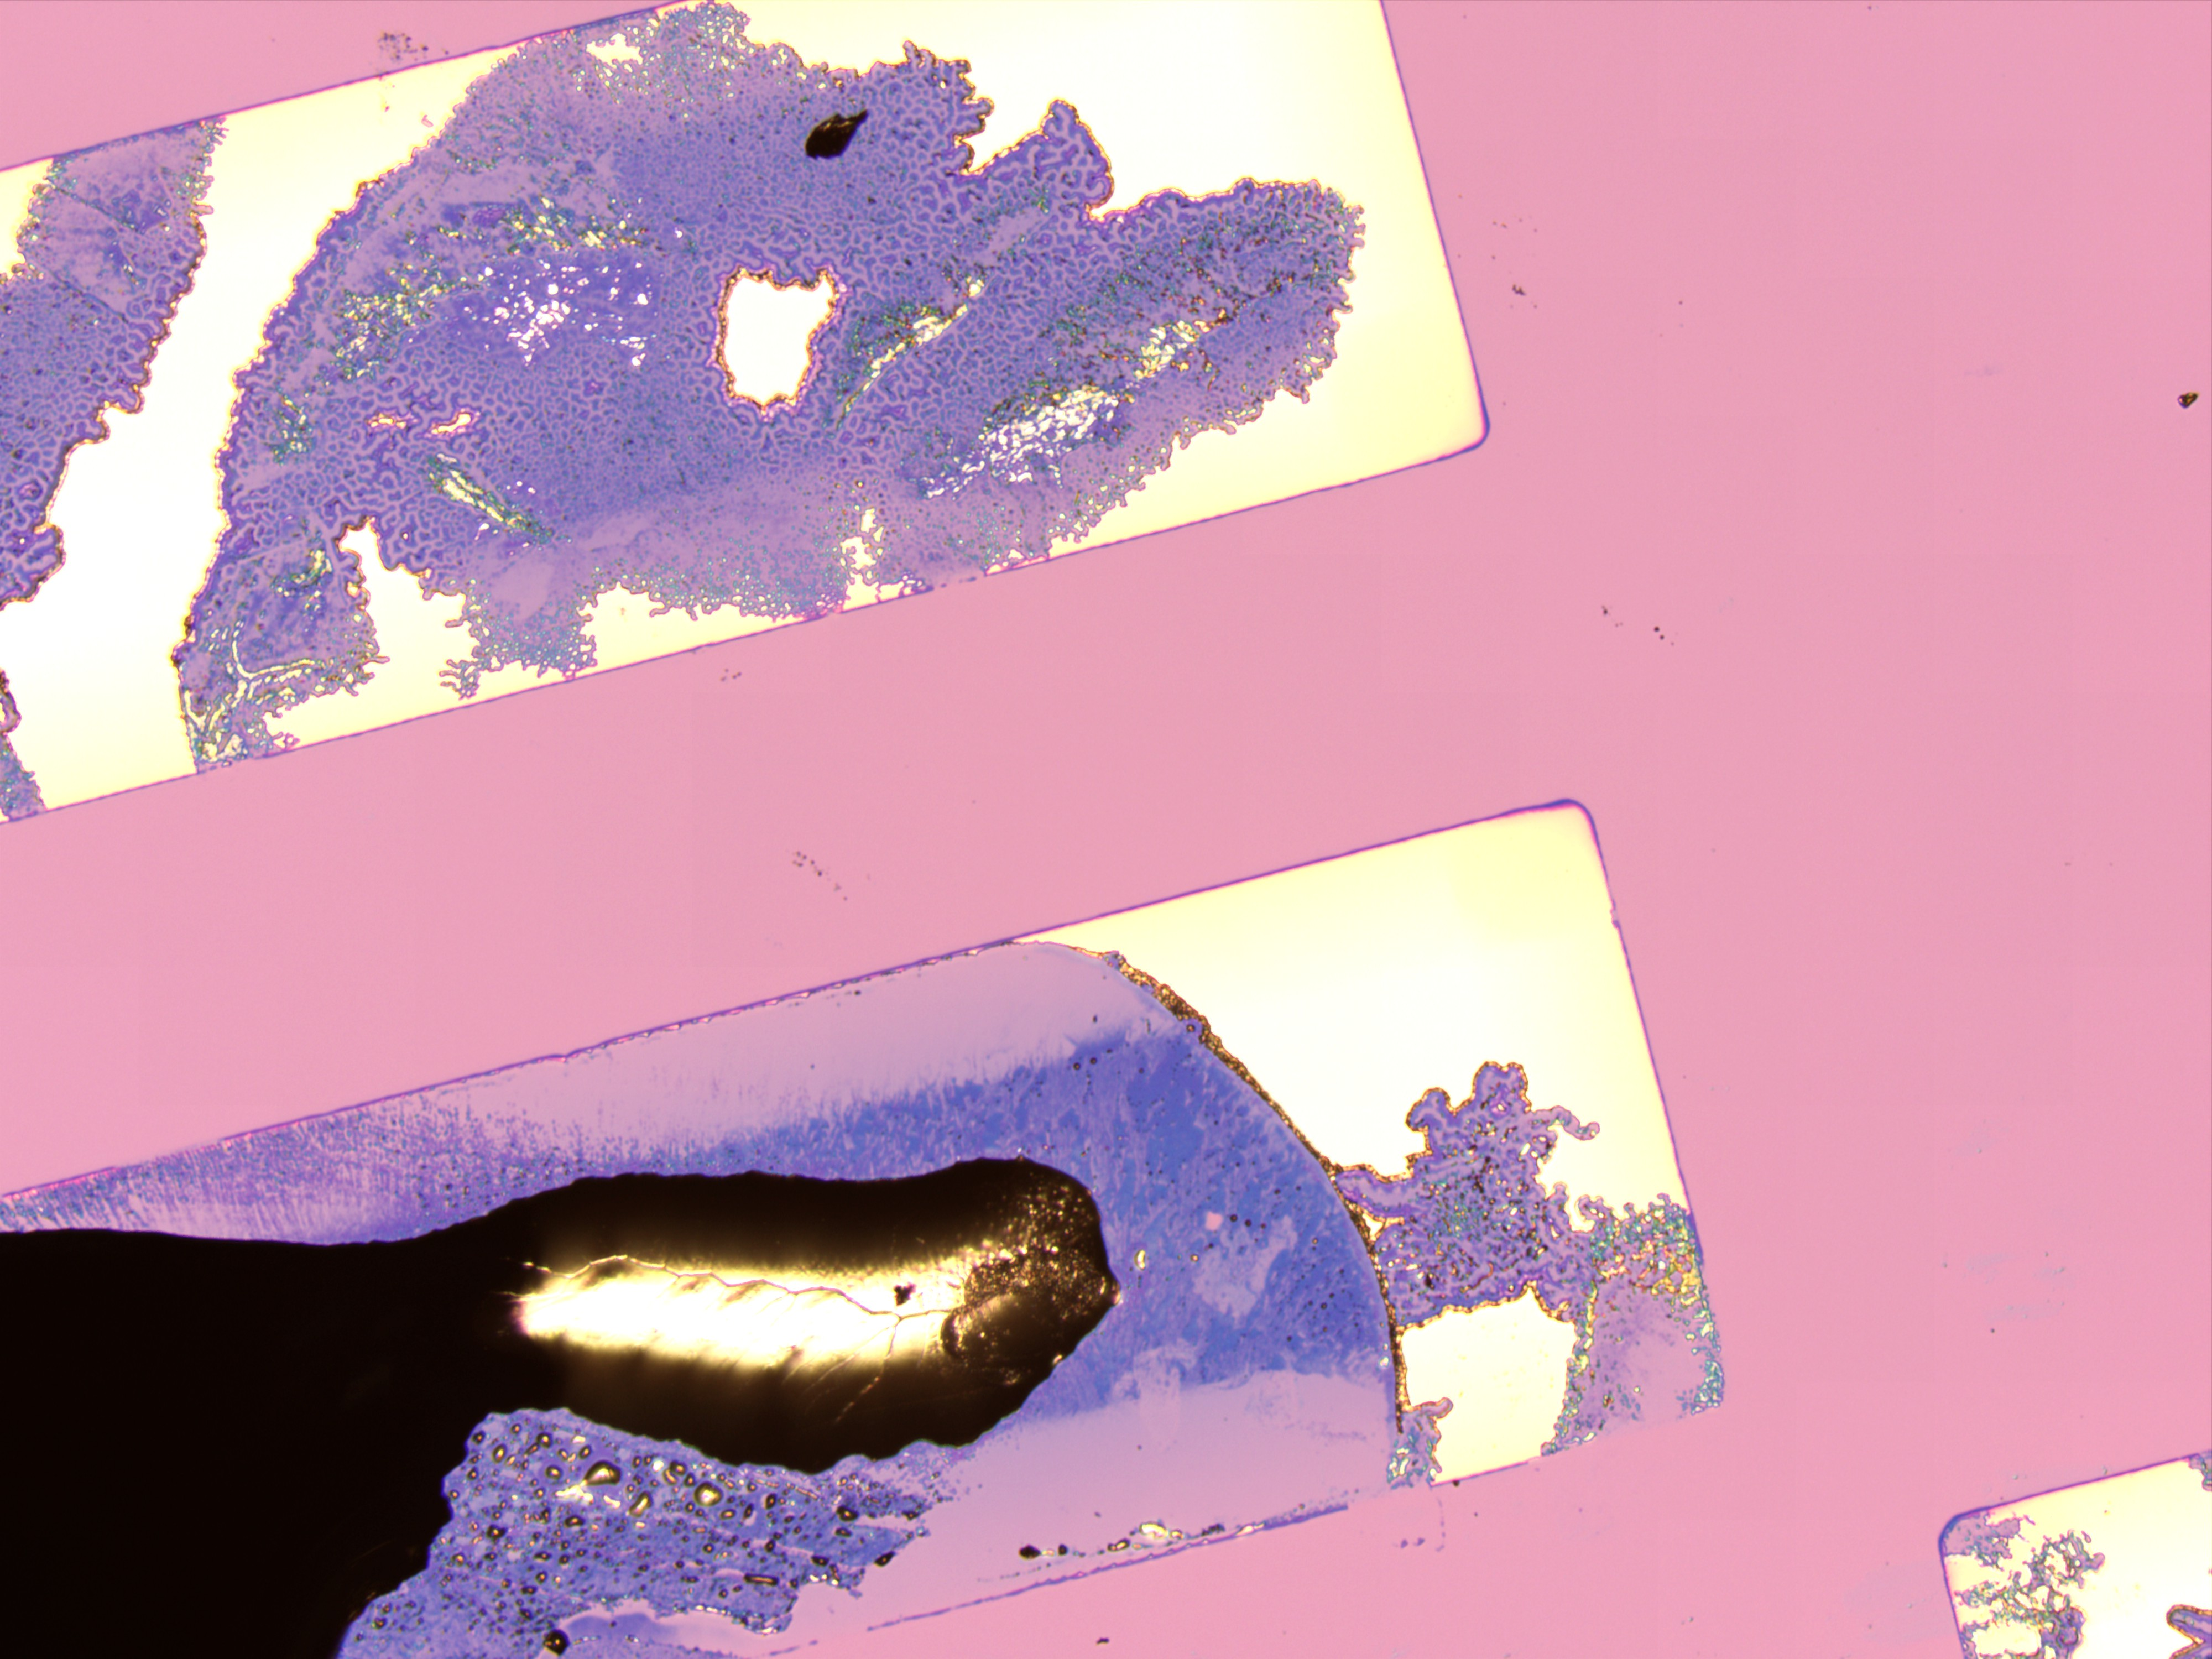
\includegraphics[width=0.85\textwidth,angle=0]{chap5/al2o3/gtransfer1}
				\caption{Adhesion of gallium to gold pads}\label{fig:al2o3_g1}
			\end{subfigure}
			\begin{subfigure}[t]{0.5\textwidth}
				\centering
				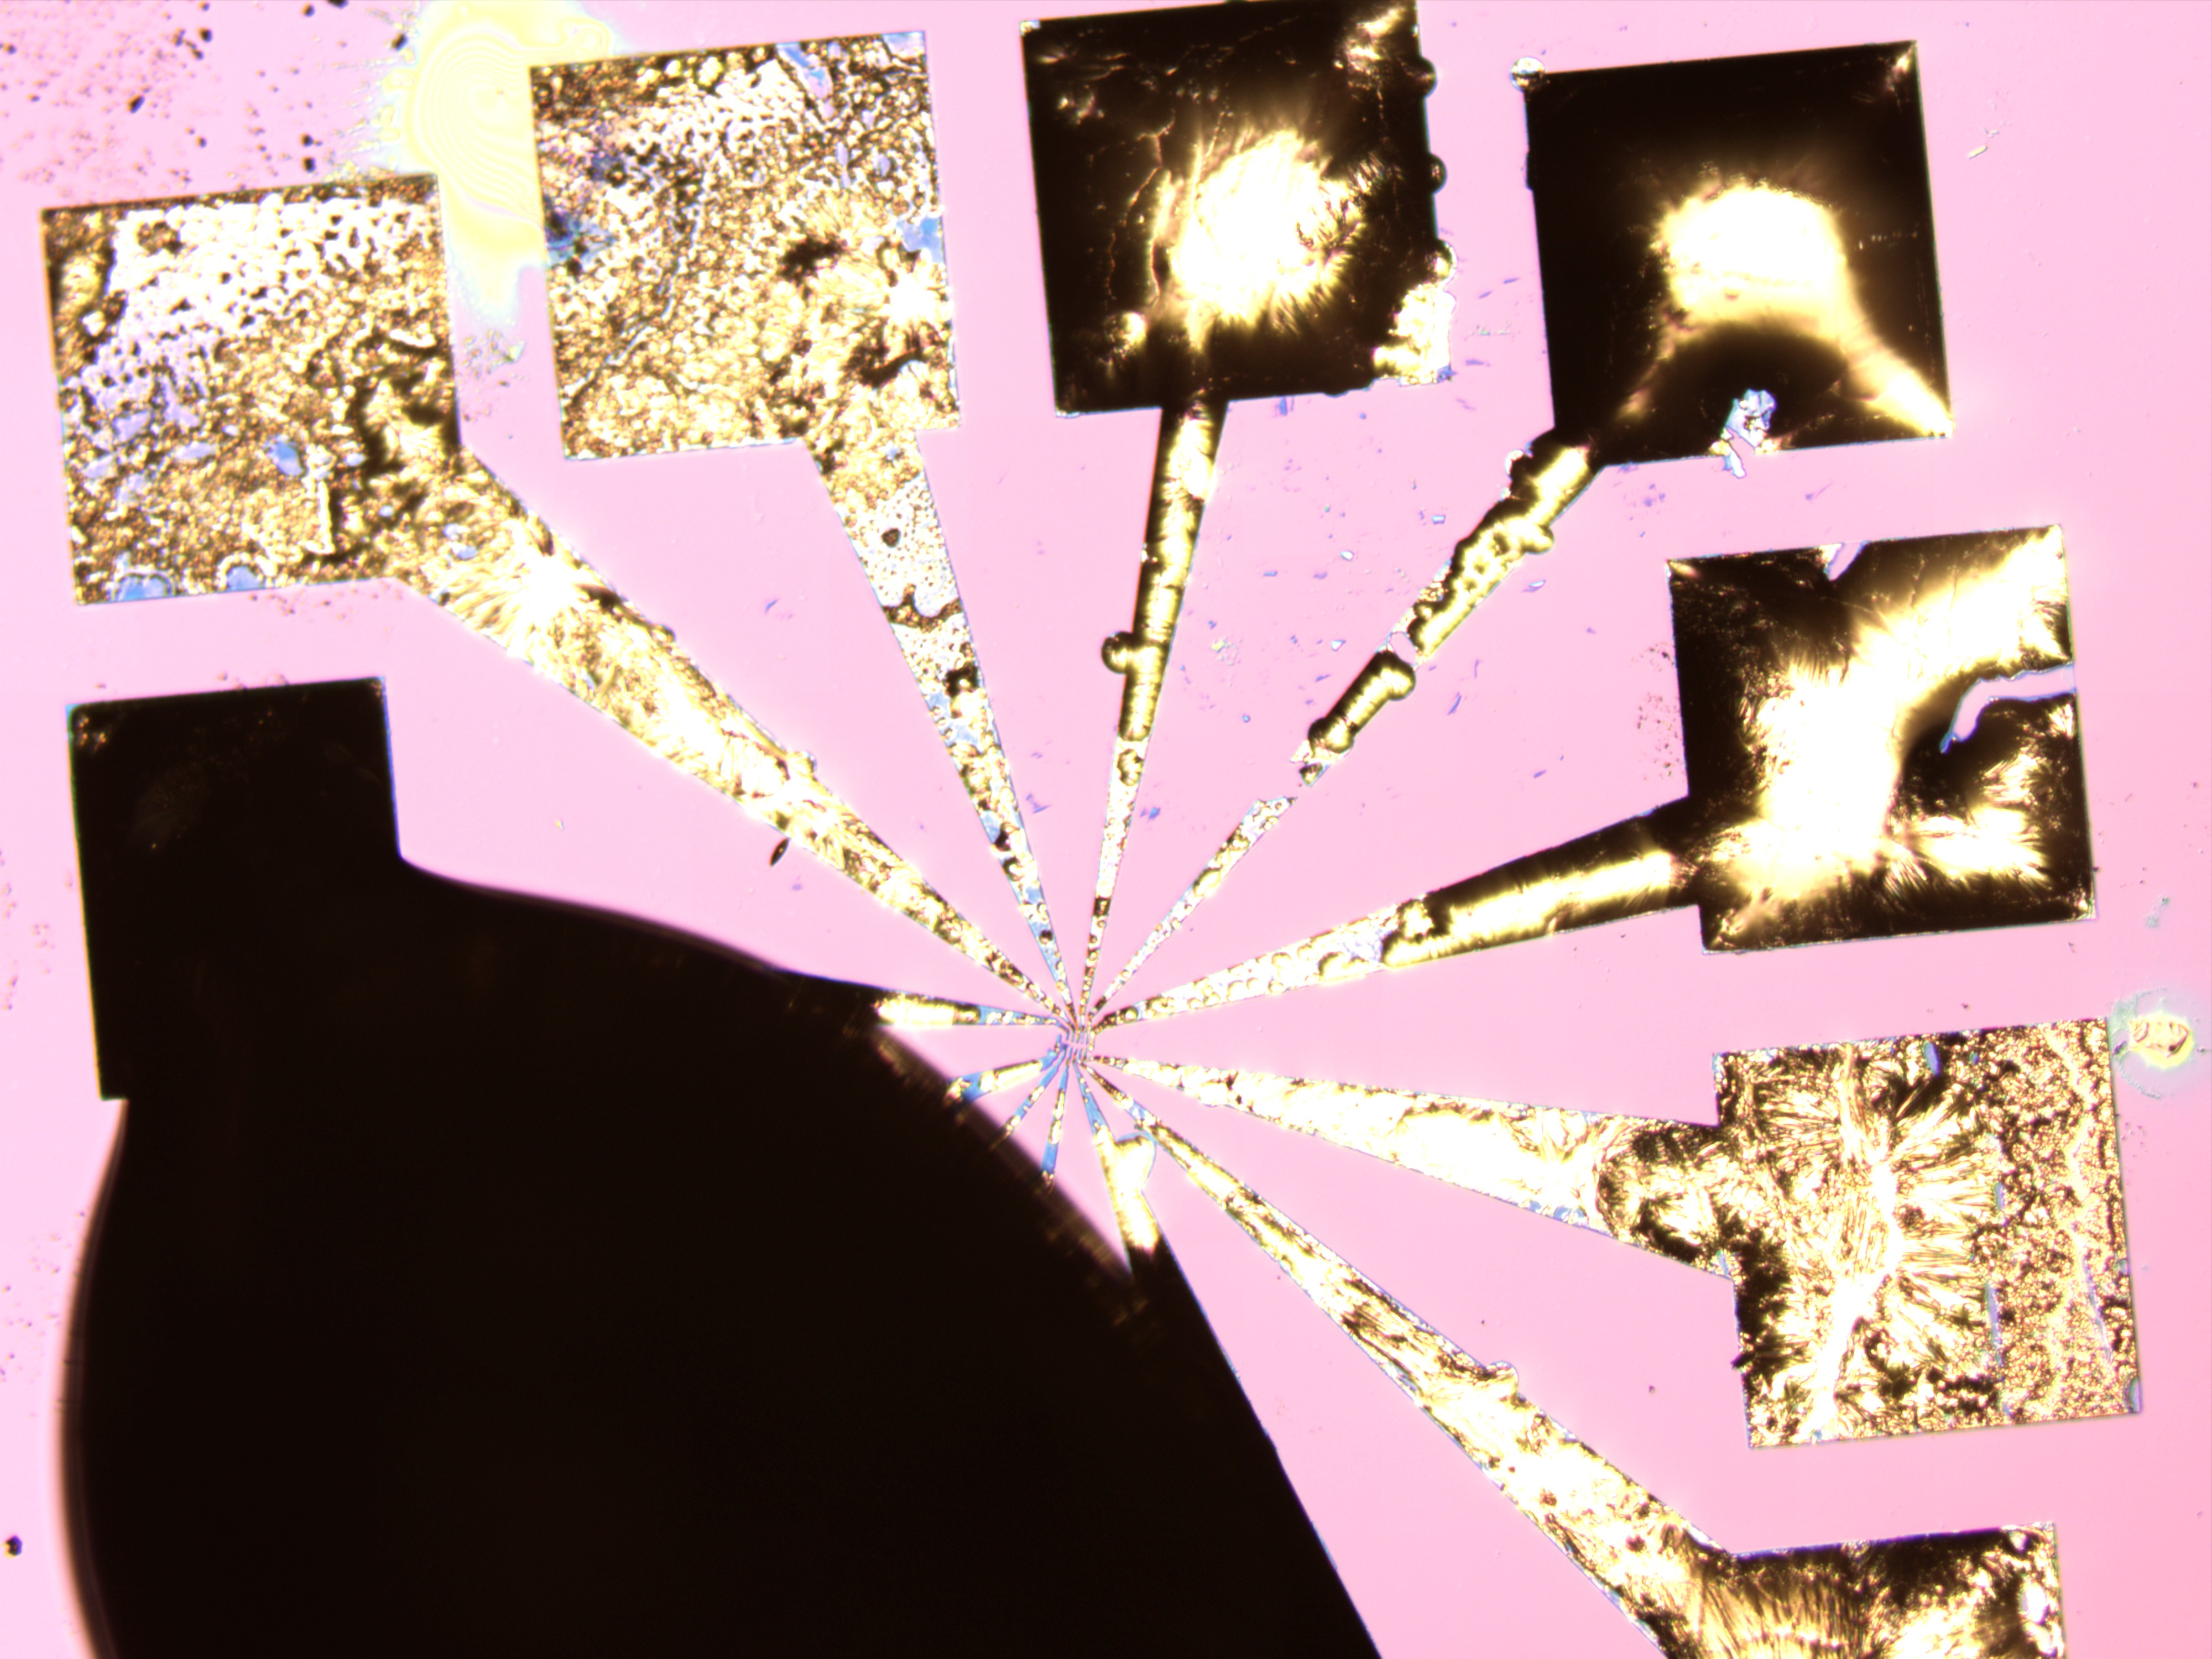
\includegraphics[width=0.85\textwidth,angle=0]{chap5/al2o3/gtransfer2}
				\caption{After cleaning off gallium, remains of gold pads}\label{fig:al2o3_g2}
			\end{subfigure}
		\end{figure}
		\begin{figure}[H]
			\ContinuedFloat
			\begin{subfigure}[t]{0.5\textwidth}
				\centering
				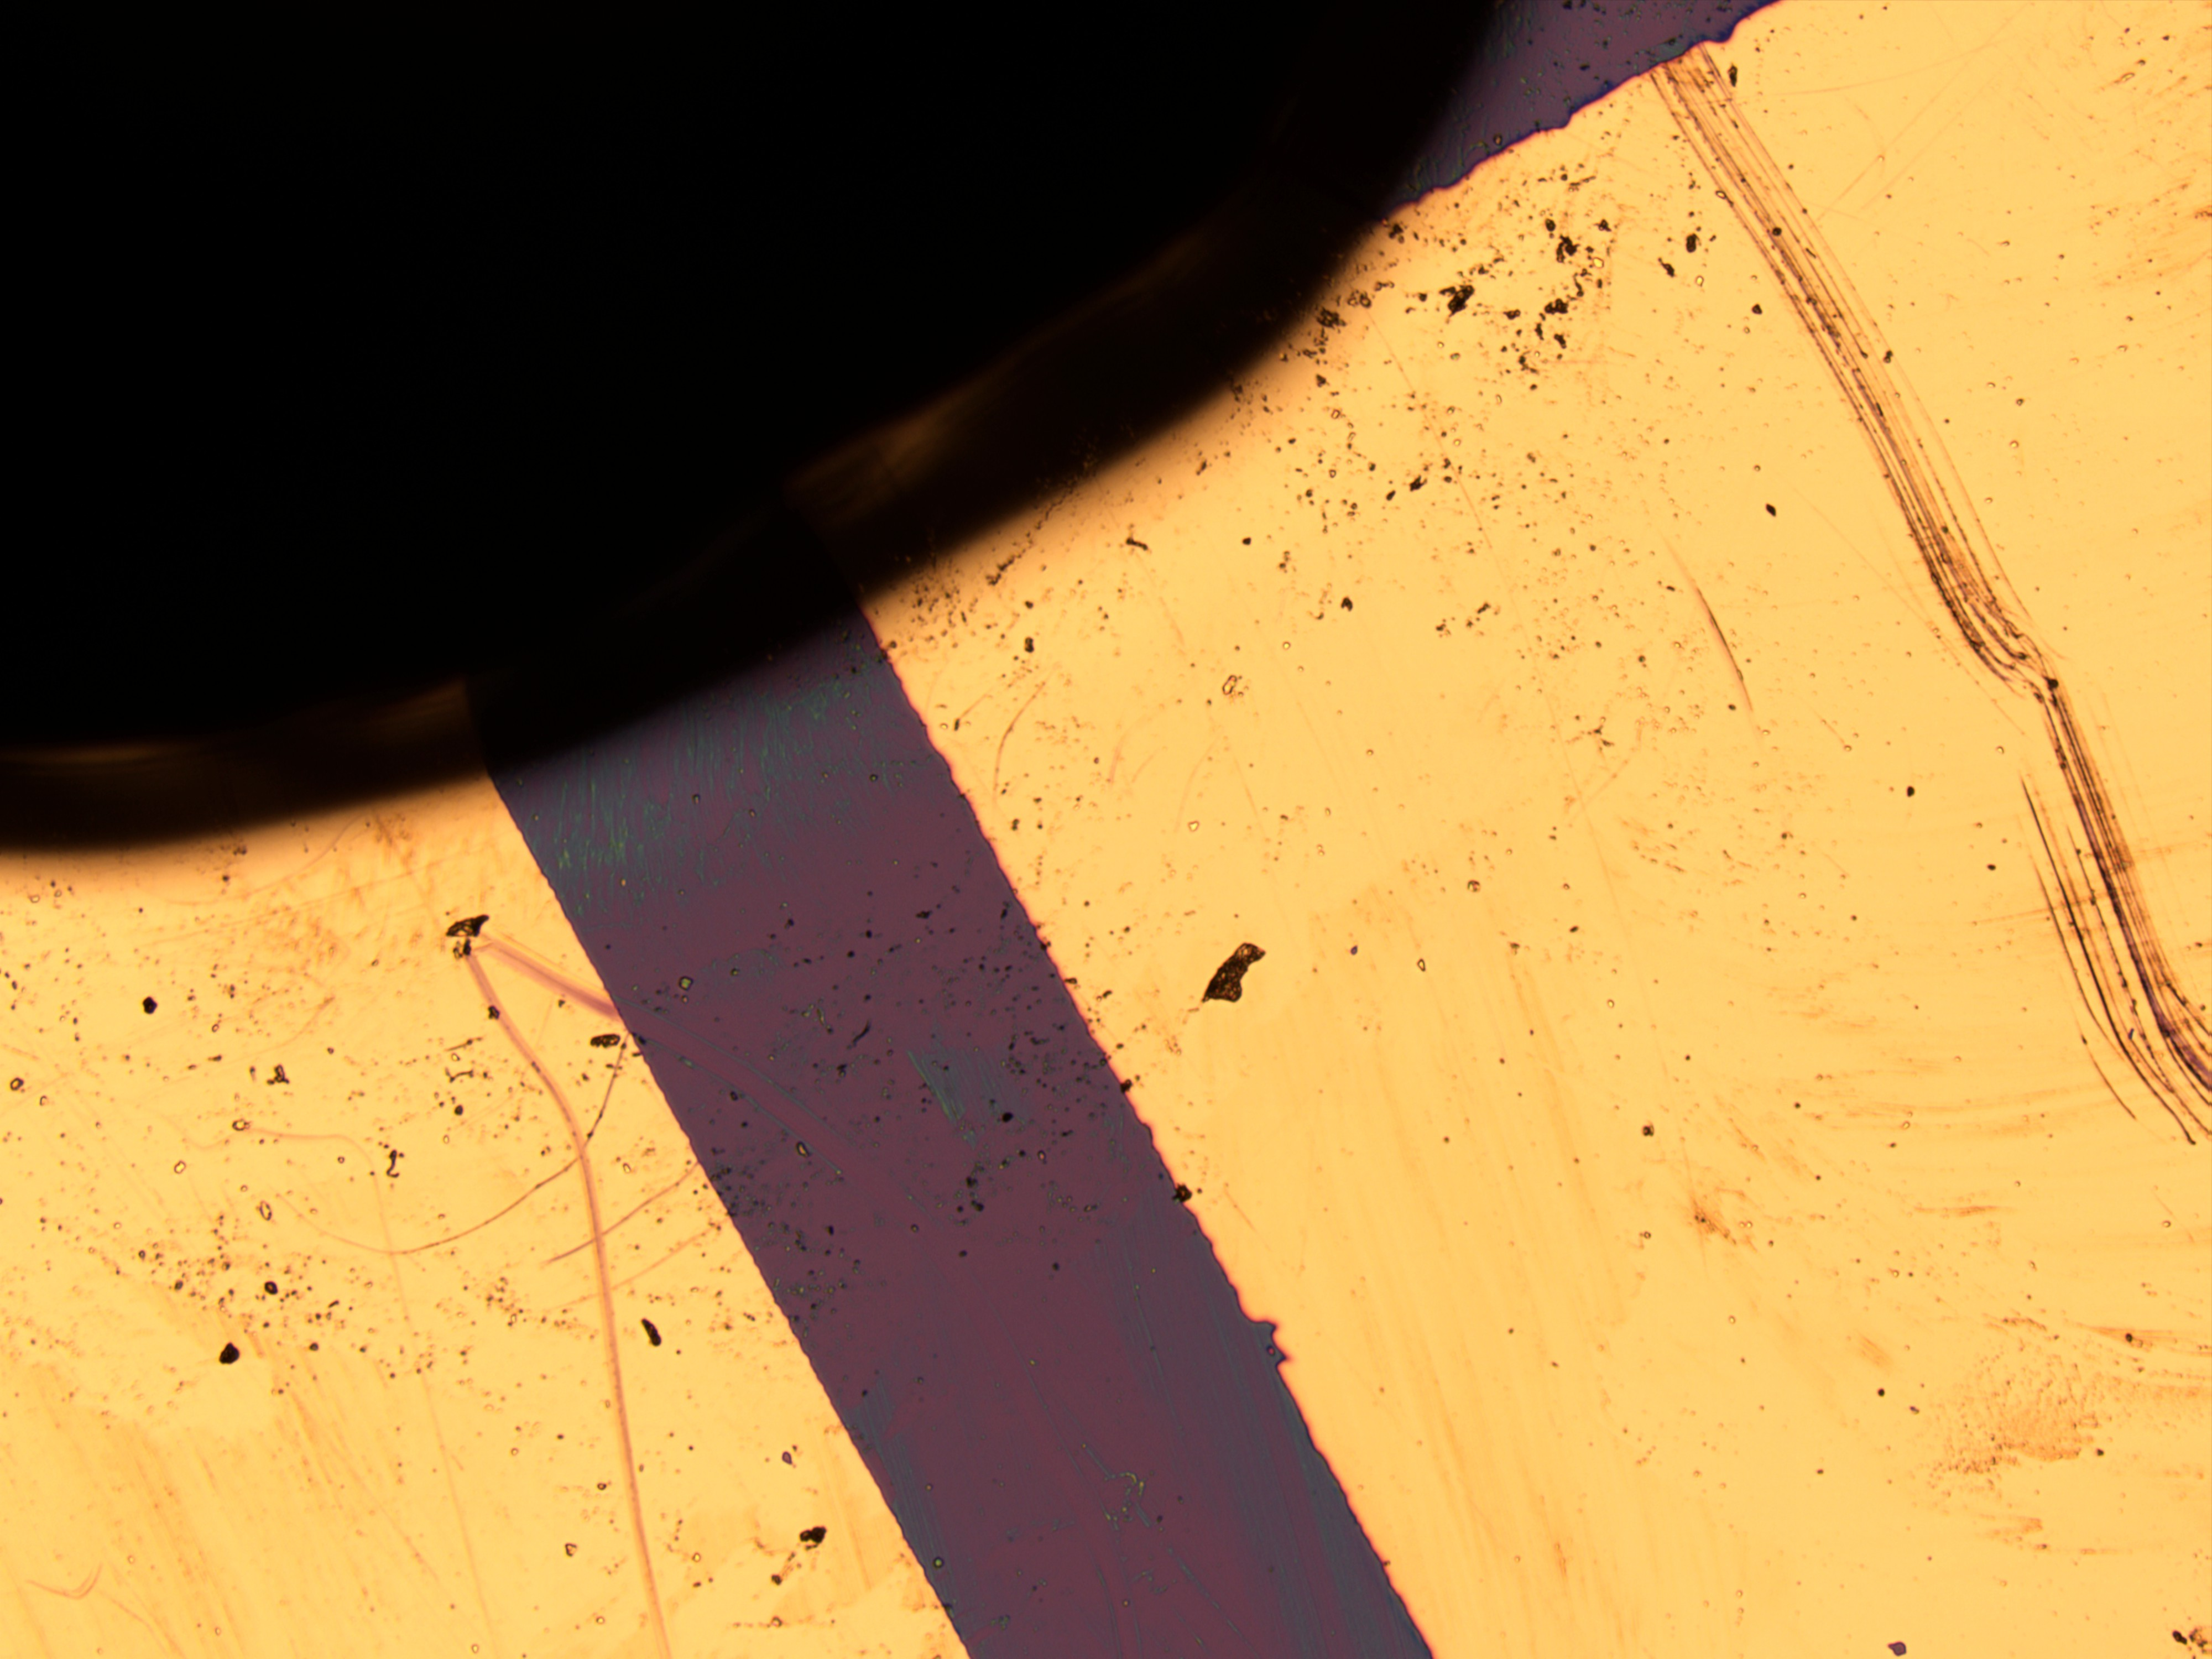
\includegraphics[width=0.85\textwidth,angle=0]{chap5/al2o3/gtransfer3}
				\caption{No oxide deposition, but surface contamination}\label{fig:al2o3_g3}
			\end{subfigure}
			\begin{subfigure}[t]{0.5\textwidth}
				\centering
				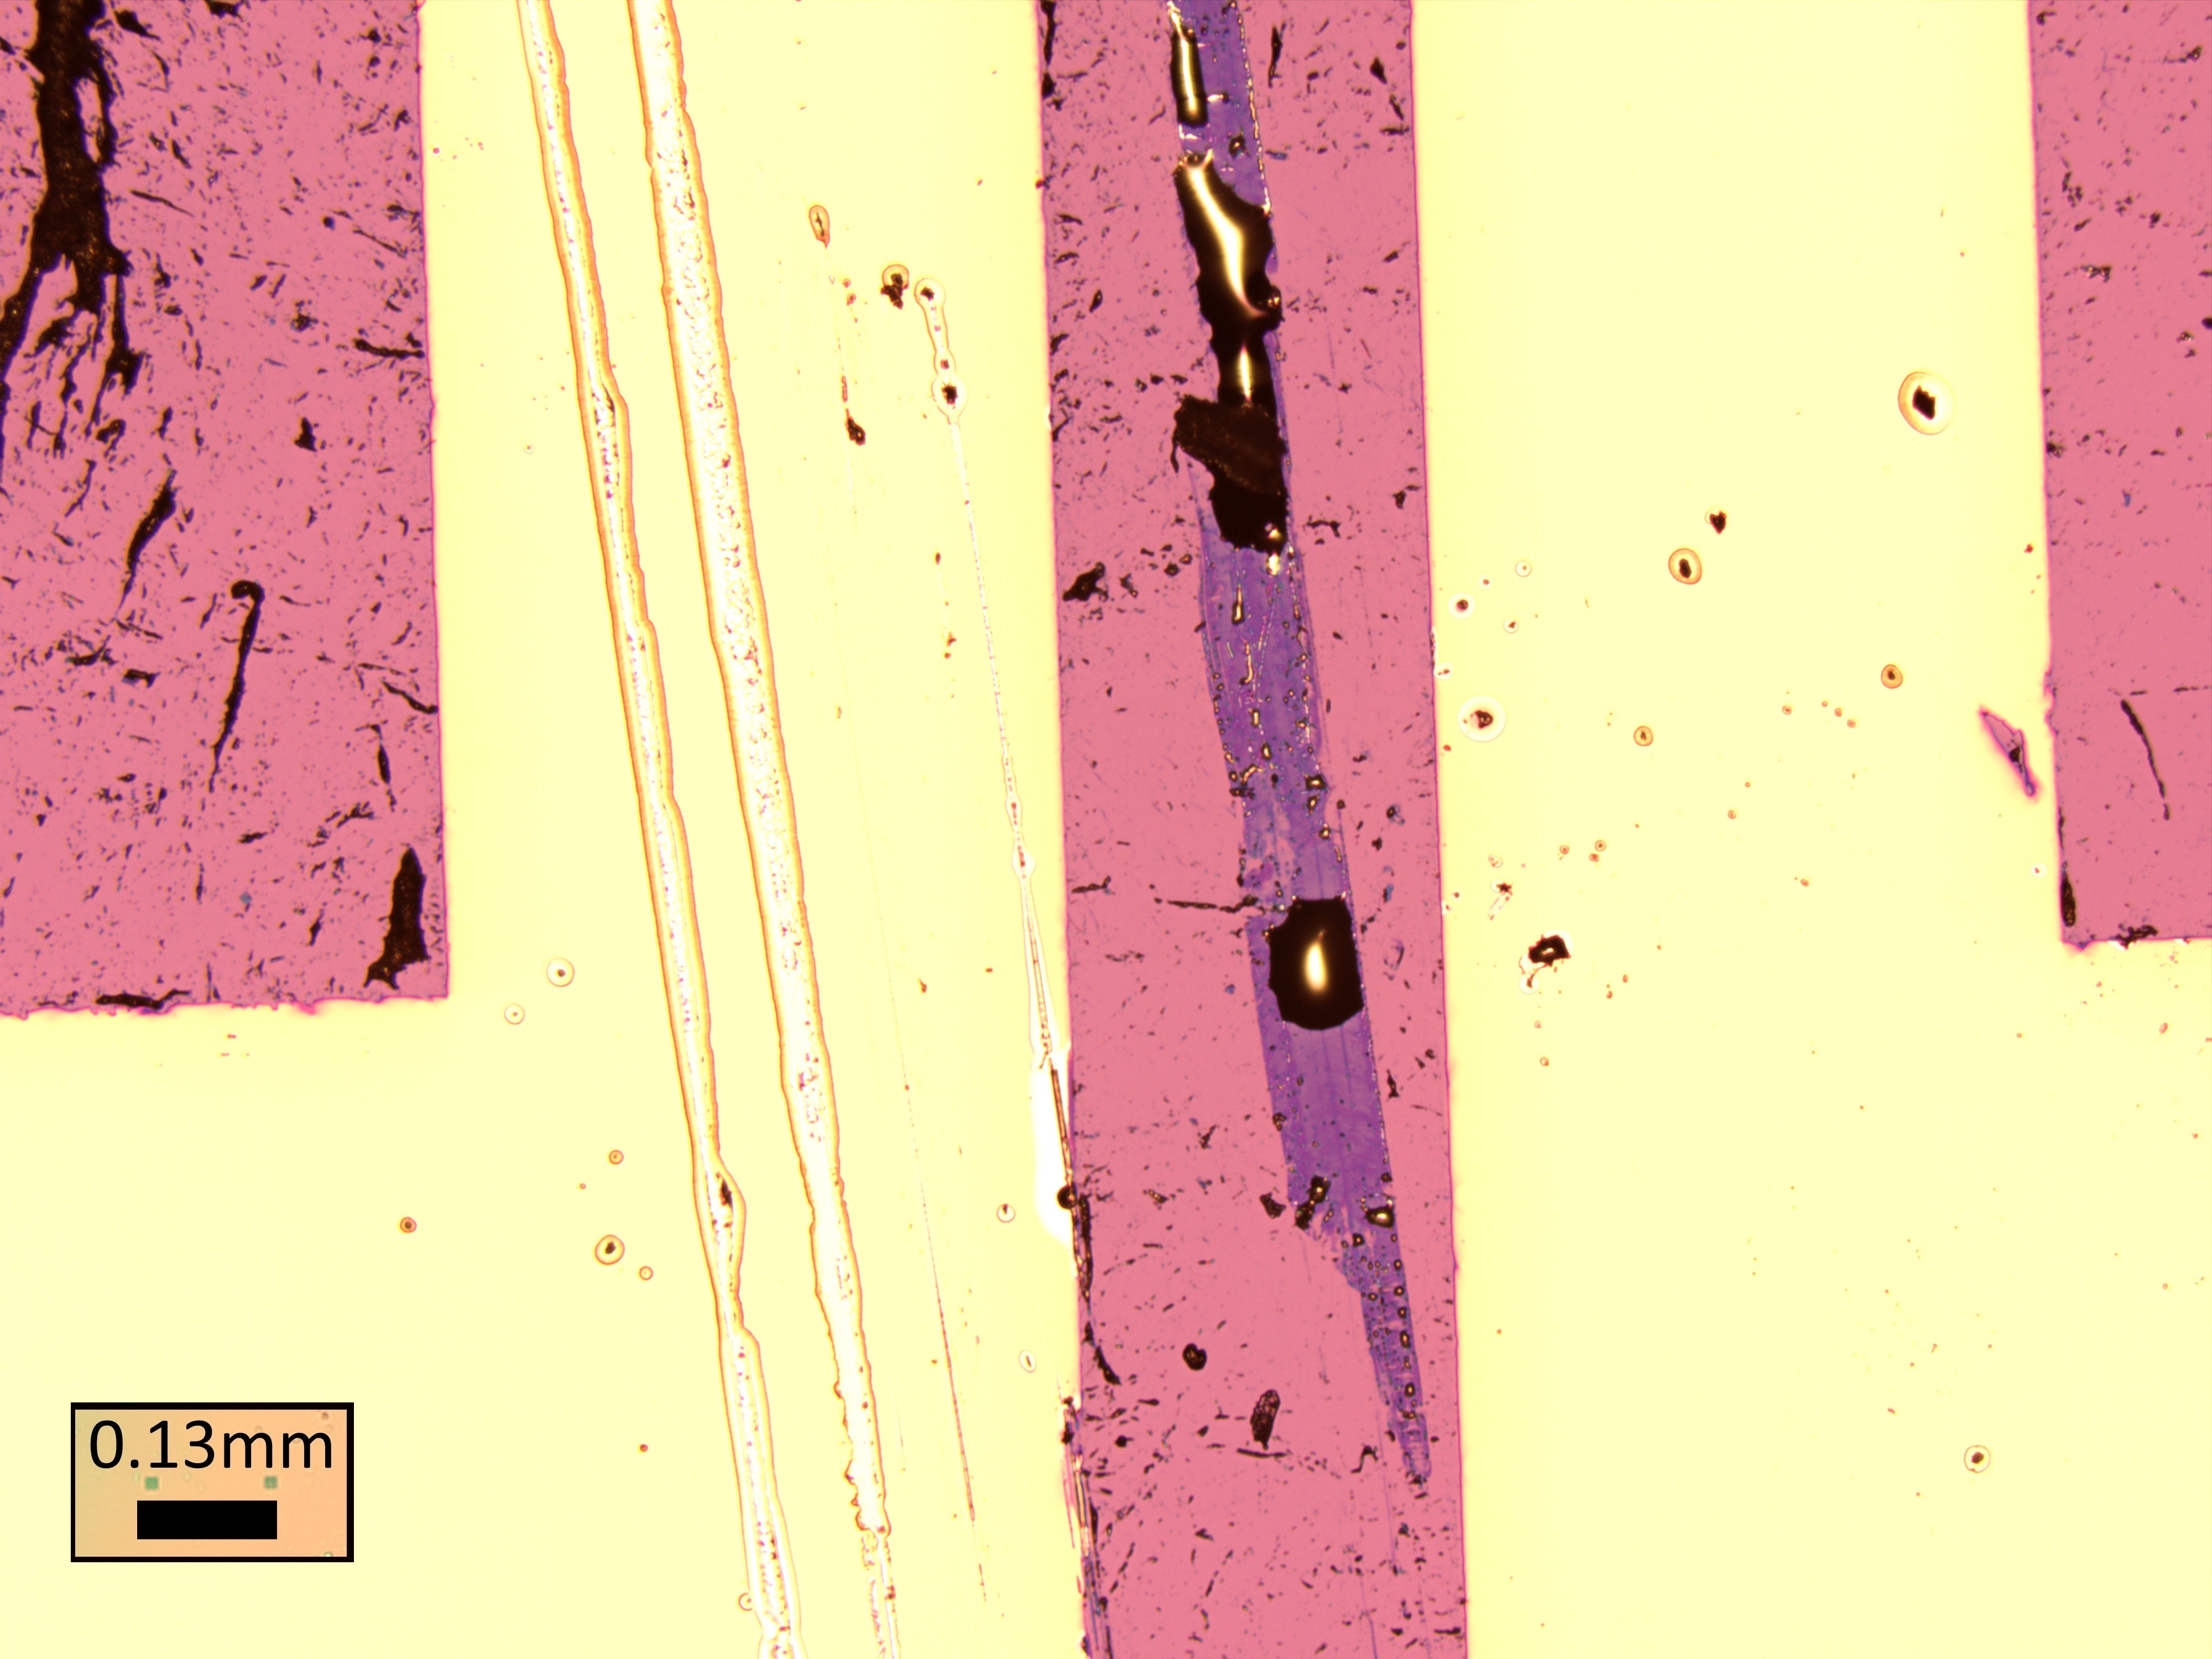
\includegraphics[width=0.85\textwidth,angle=0]{chap5/al2o3/gtransfer4}
				\caption{Gallium metal and some gallium oxide deposition}\label{fig:al2o3_g4}
			\end{subfigure}
			\caption[\aluminimumoxide{} stamped on \silicondioxide{}]{Deposition of \aluminimumoxide{} onto Au on \silicondioxide{}}\label{fig:transfer_al_on_au&si}
		\end{figure}
		We also attempted spreading oxide on transferred CVD graphene, but no evidence of oxide transfer was found optically (\cref{fig:transfer_al_on_cvd}).
		\begin{figure}[H]
			\begin{subfigure}[t]{0.5\textwidth}
				\centering
				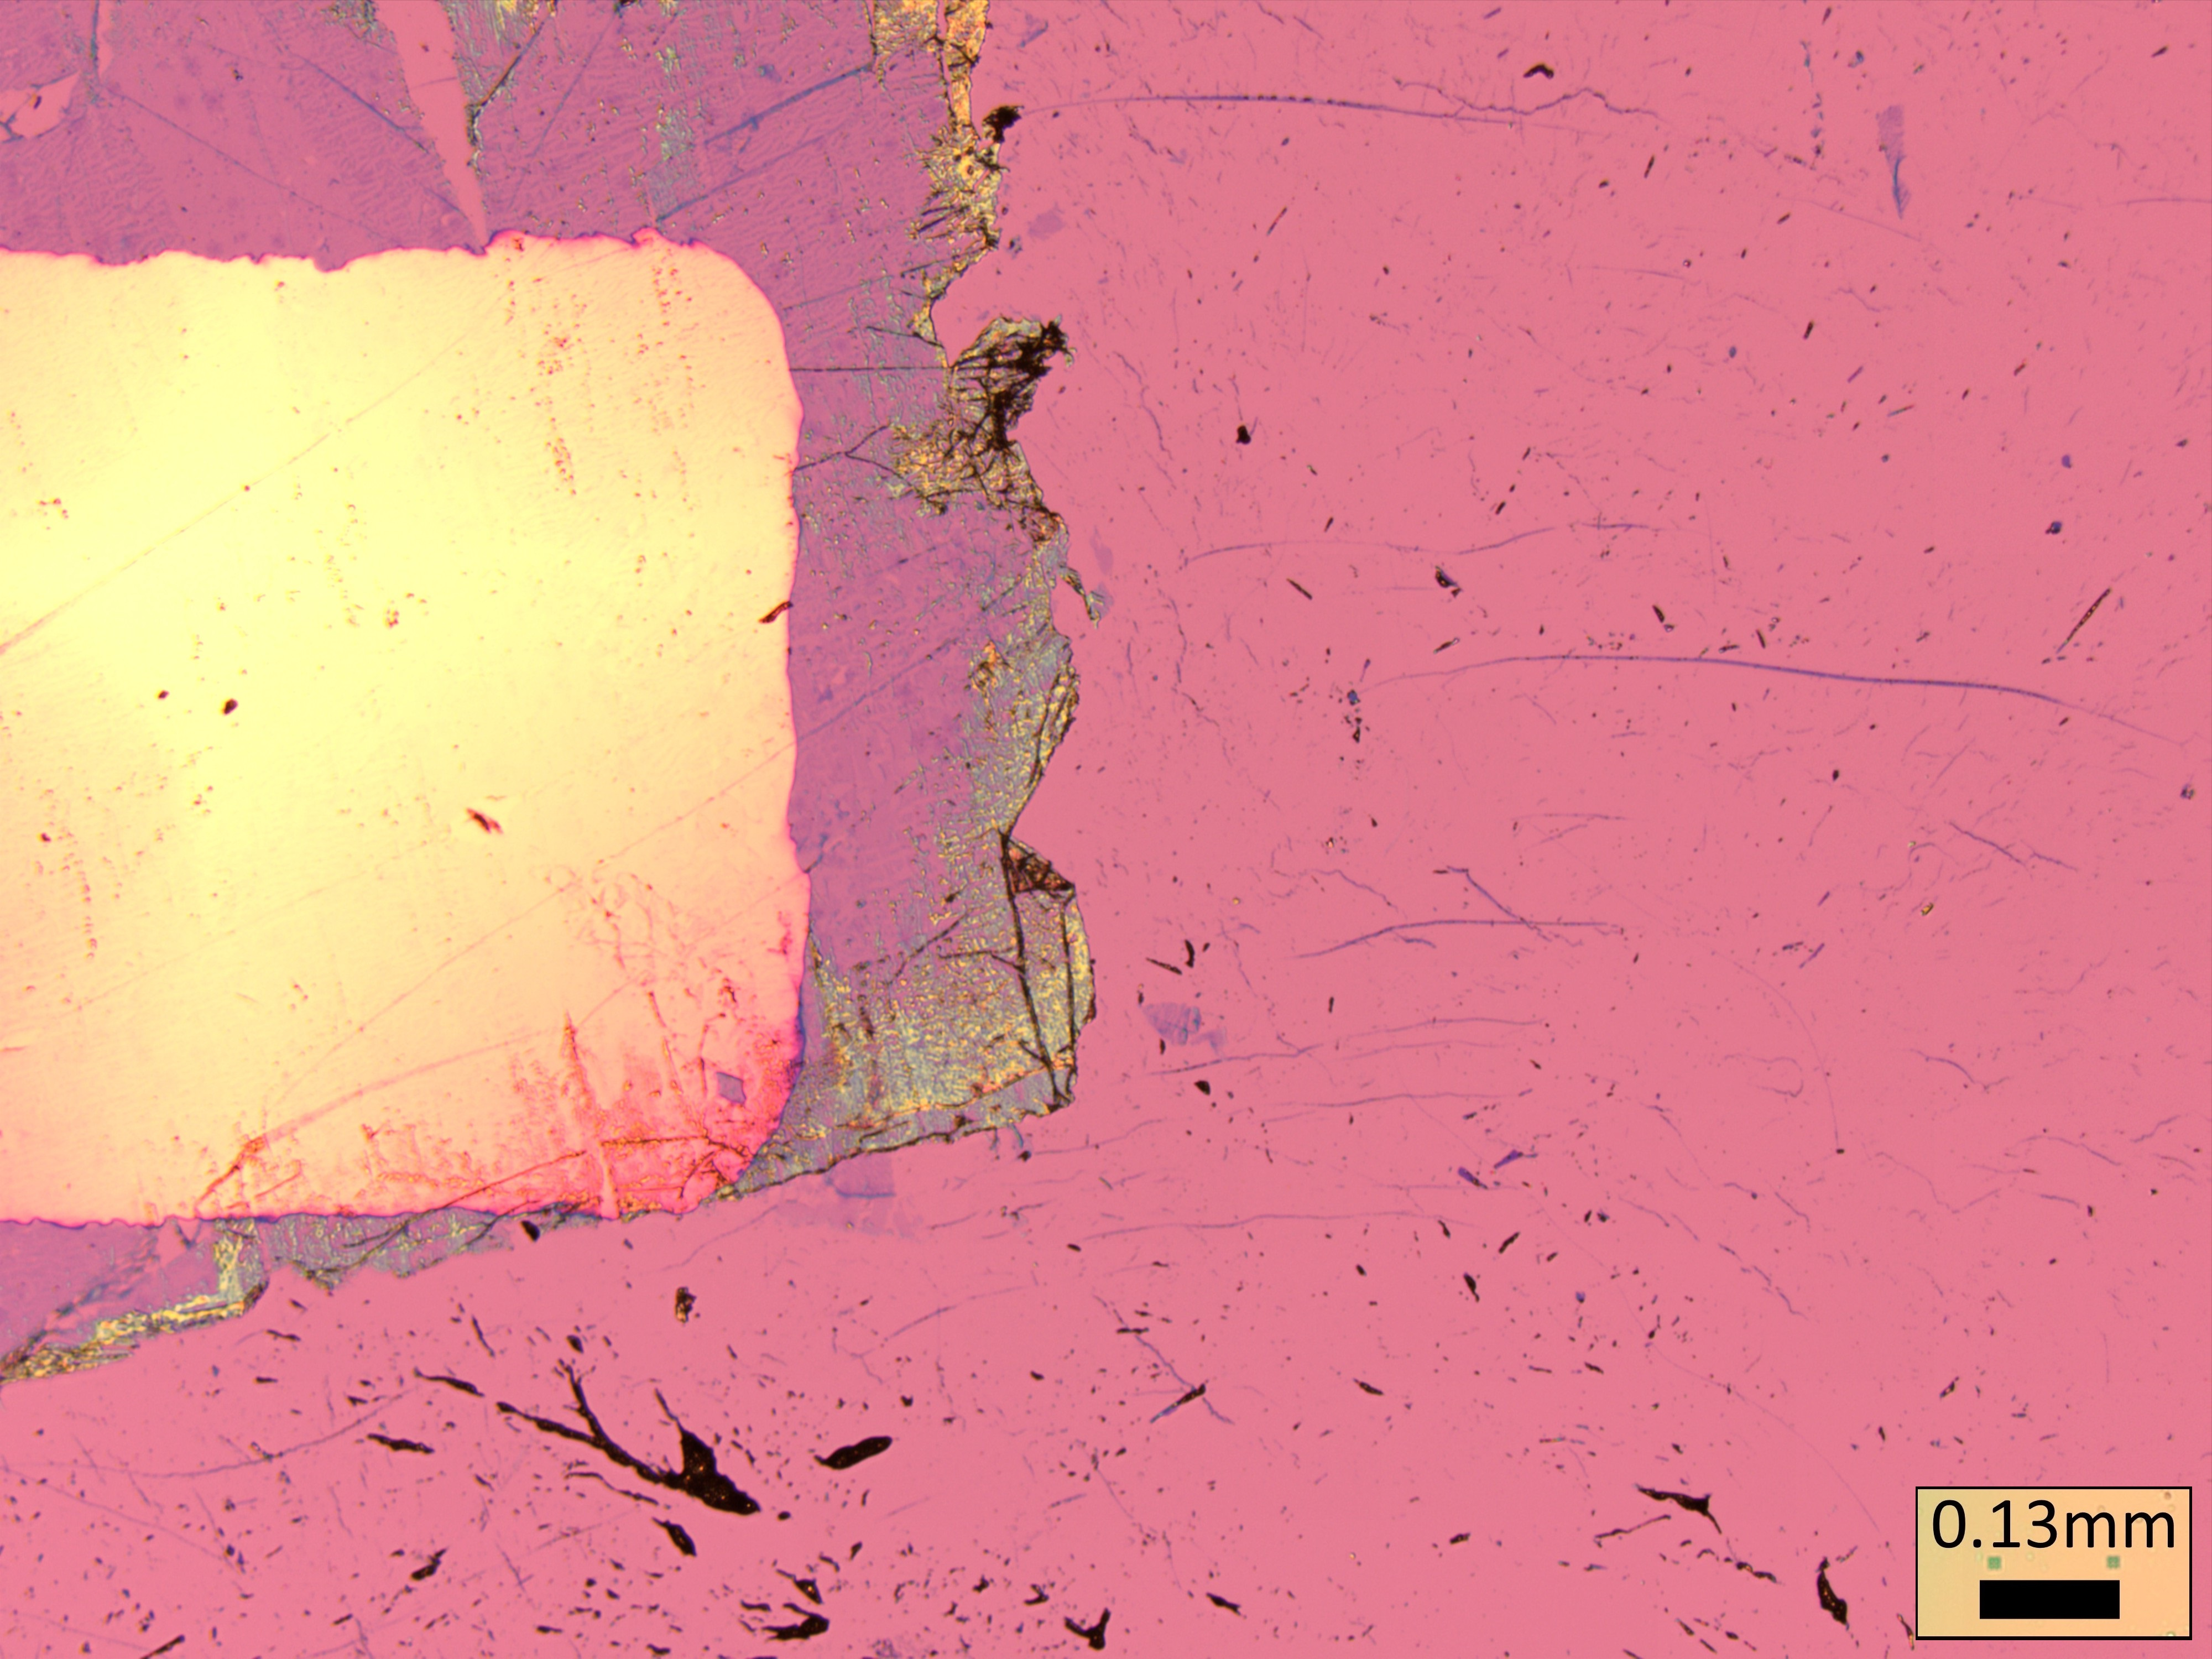
\includegraphics[width=0.85\textwidth,angle=0]{chap5/al2o3/ctransfer1}
				\caption{}\label{fig:al2o3_c1}
			\end{subfigure}
			\begin{subfigure}[t]{0.5\textwidth}
				\centering
				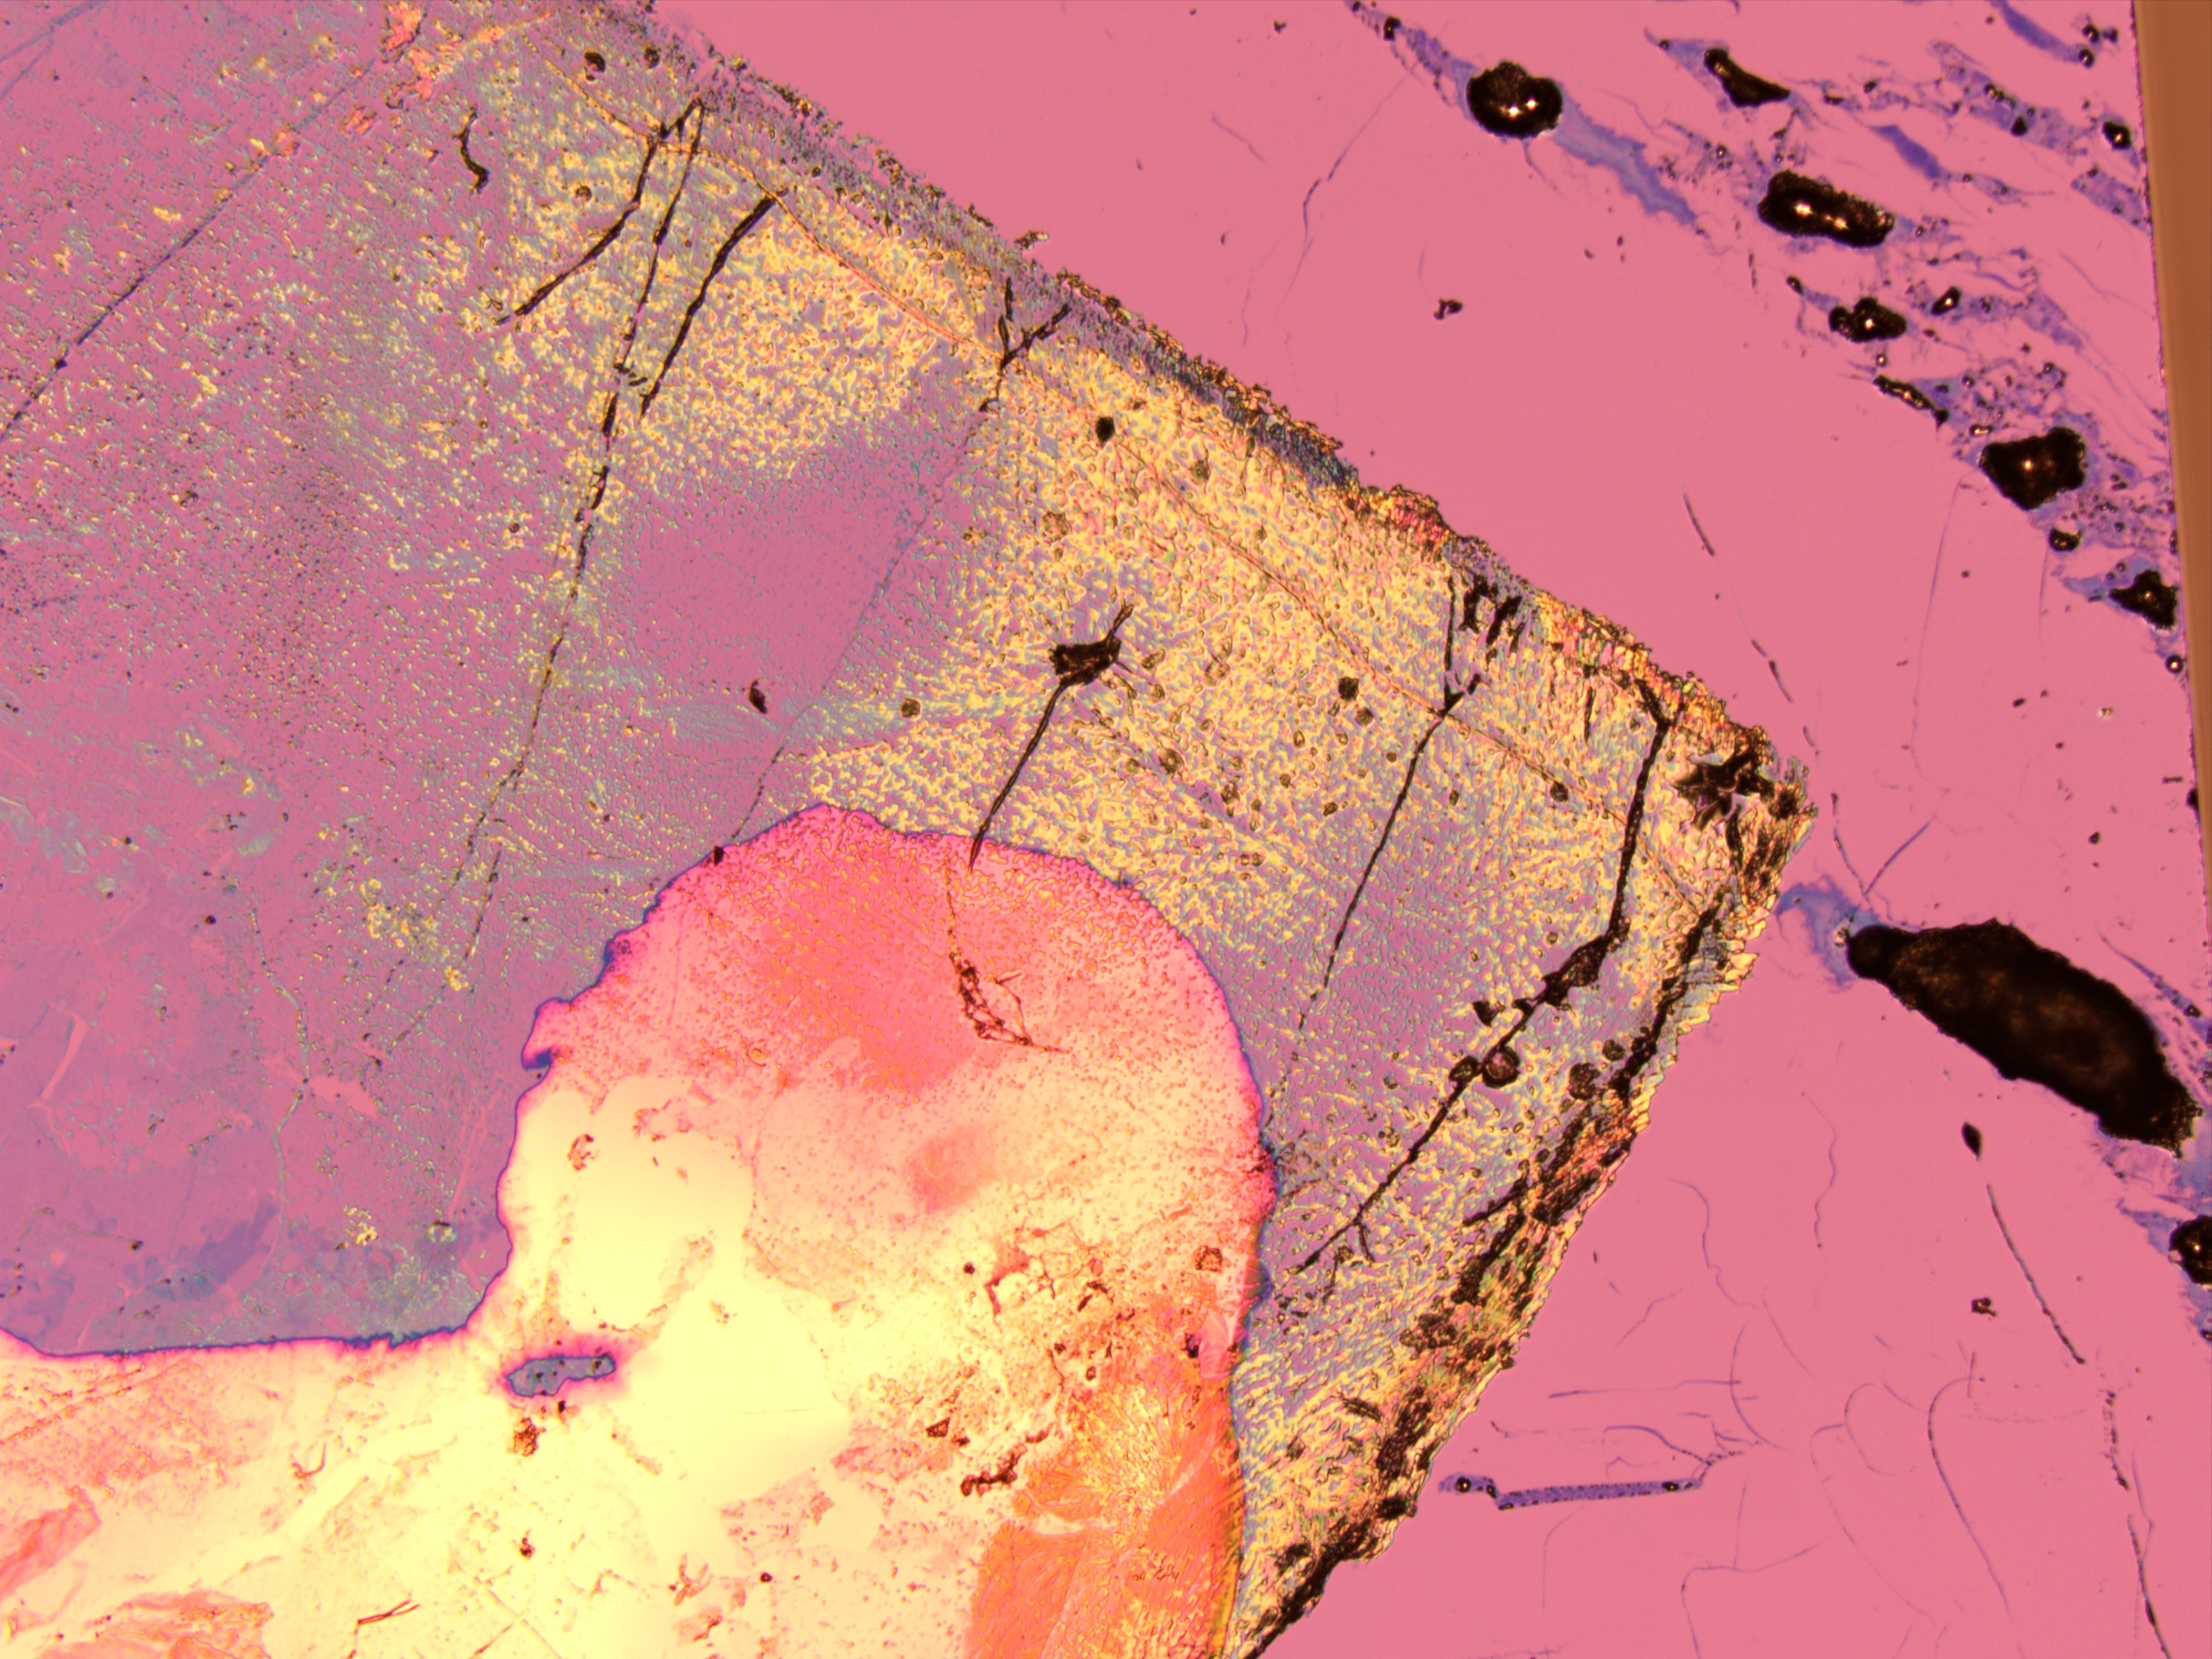
\includegraphics[width=0.85\textwidth,angle=0]{chap5/al2o3/ctransfer2}
				\caption{}\label{fig:al2o3_c2}
			\end{subfigure}
			\caption[\aluminimumoxide{} stamped on CVD graphene \& \silicondioxide{}]{Contamination of CVD graphene without transfer of \aluminimumoxide{}.}\label{fig:transfer_al_on_cvd}
		\end{figure}
		After three trials using aluminium oxide and varying the exfoliation method, Torben suggested we try some other oxides for something more reliable and clean, particularly for the time window of this project. 
	
	\subsection{SnO \& Bi$_2$O$_3$}
	After switching away from \aluminimumoxide{}, I tried to start using \tinoxide{}, \bismuthoxide{} and \galliumoxide{}. Hareem assisted me with transfering \bismuthoxide{} and \tinoxide{} onto desired substrates, using the same base method of exfoliation in a low oxygen fumehood, but with a few modifications. 
	
	Different from \aluminimumoxide{}, we used pure tin and bismuth (no need for a gallium alloy) and melted the chunks on a hotplate at 330 $^\circ$C and 270 $^\circ$C  respectively. We also used glass slides to `sacrifice' a layer of outer material before proceeding to attempt to exfoliate a layer of material.
	
	We had immediate success with this method for depositing onto bare substrates, as seen in \cref{fig:transfer_bi&sno_on_si}.
	\begin{figure}[H]
		\begin{subfigure}[t]{0.24\textwidth}
			\centering
			\includegraphics[width=0.95\textwidth,angle=0]{chap5/bi2o3/transfer1}
			\caption{Clean \bismuthoxide{} sheet - 5x}\label{fig:bi2o3_1}
		\end{subfigure}
		\begin{subfigure}[t]{0.24\textwidth}
			\centering
			\includegraphics[width=0.95\textwidth,angle=0]{chap5/bi2o3/transfer1_50x}
			\caption{Clean \bismuthoxide{} sheet - 50x}\label{fig:bi2o3_2}
		\end{subfigure}
		\begin{subfigure}[t]{0.24\textwidth}
			\centering
			\includegraphics[width=0.95\textwidth,angle=0]{chap5/sno/transfer1}
			\caption[\tinoxide{} transfer on \silicondioxide{}]{A clean transfer of \tinoxide{} onto \silicondioxide{} 5x}\label{fig:sno_1}
		\end{subfigure}
		\begin{subfigure}[t]{0.24\textwidth}
			\centering
			\includegraphics[width=0.95\textwidth,angle=0]{chap5/sno/transfer1_50x}
			\caption{Clean \tinoxide{} transfer 50x}\label{fig:sno_2}
		\end{subfigure}
		\begin{subfigure}[t]{0.24\textwidth}
			\centering
			\includegraphics[width=0.95\textwidth,angle=0]{chap5/bi2o3/transfer2}
			\caption{\bismuthoxide{} with nearby metal - 5x}\label{fig:bi2o3_3}
		\end{subfigure}
		\begin{subfigure}[t]{0.24\textwidth}
			\centering
			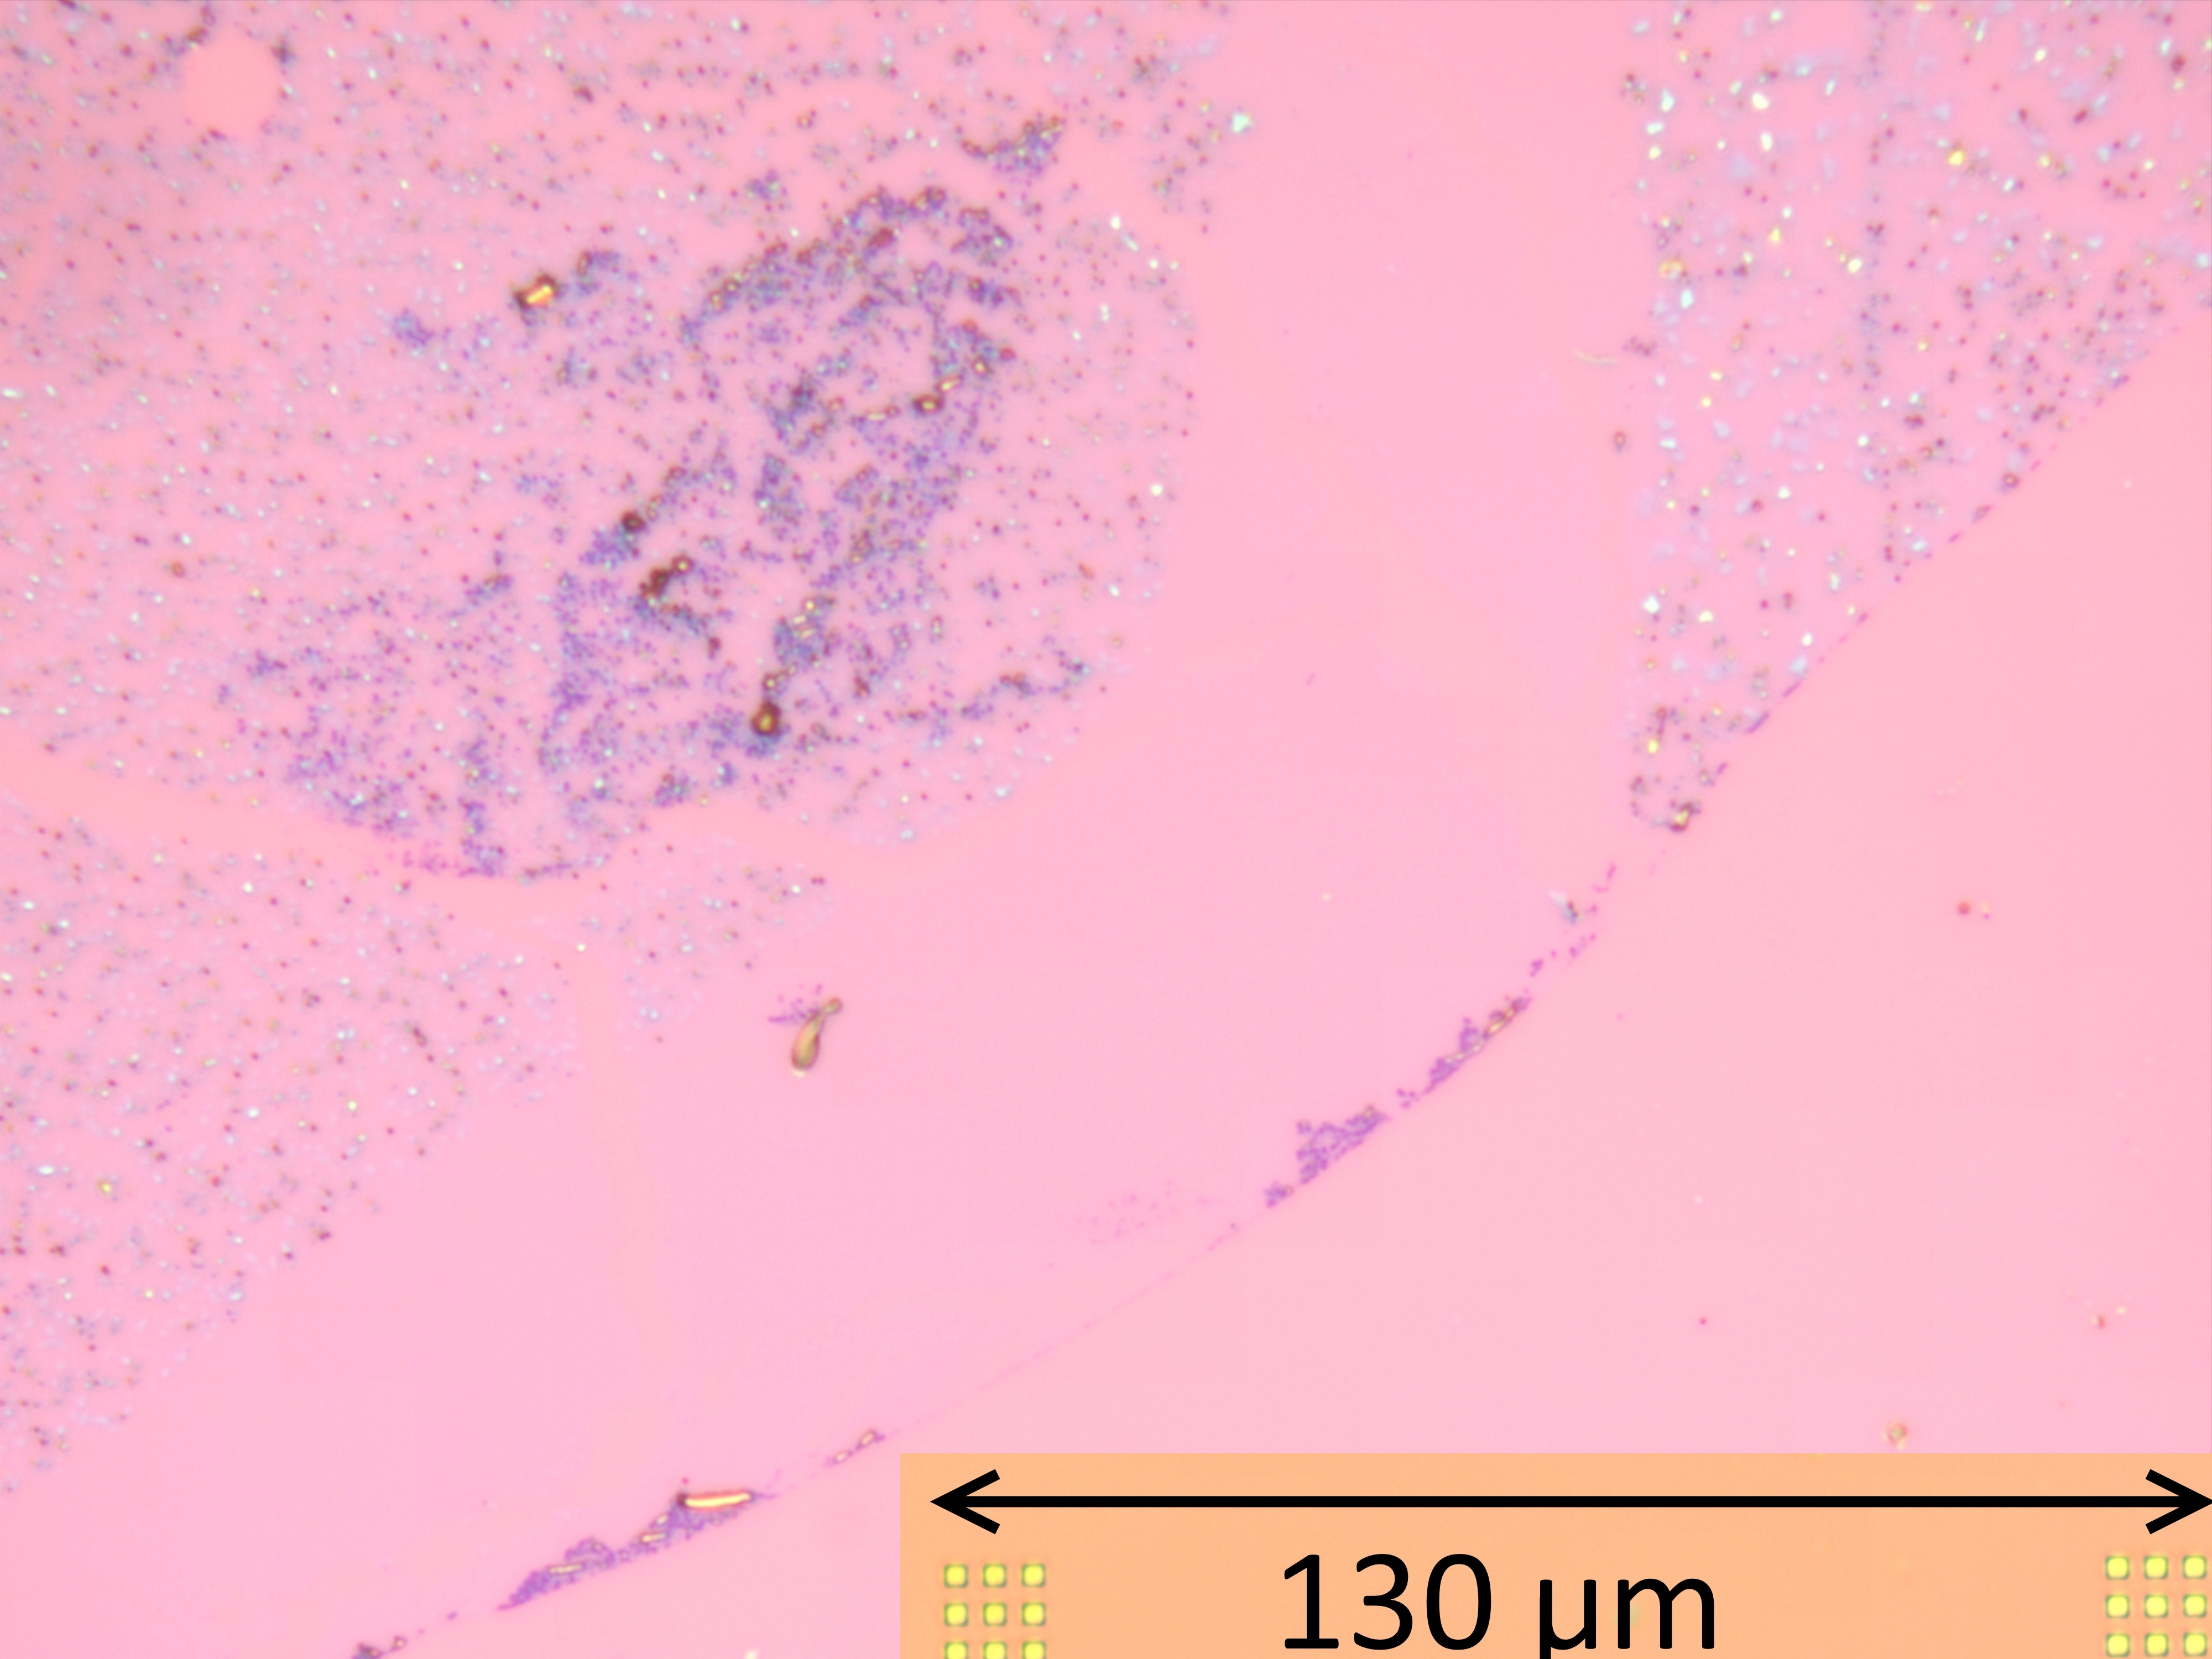
\includegraphics[width=0.95\textwidth,angle=0]{chap5/bi2o3/transfer2_50x}
			\caption{\bismuthoxide{} with nearby metal - 50x}\label{fig:bi2o3_4}
		\end{subfigure}
		\begin{subfigure}[t]{0.24\textwidth}
			\centering
			\includegraphics[width=0.95\textwidth,angle=0]{chap5/sno/transfer2}
			\caption{Clean \tinoxide{} sheet with some metal remnant}\label{fig:sno_3}
		\end{subfigure}
		\begin{subfigure}[t]{0.24\textwidth}
			\centering
			\includegraphics[width=0.95\textwidth,angle=0]{chap5/sno/transfer3}
			\caption{\tinoxide{} sheet with holes}\label{fig:sno_4}
		\end{subfigure}
		\caption[\bismuthoxide{} and \tinoxide{} stamped on \silicondioxide{}]{Deposition of \bismuthoxide{} and \tinoxide{} onto \silicondioxide{}. Scale bar: 0.13mm}\label{fig:transfer_bi&sno_on_si}
	\end{figure}
	
	Sheets are much more uniform and easy to come by than that of \aluminimumoxide{}. Unfortunately it was still clear () that, for both bismuth and tin metals, adhesion to gold contacts was still a significant problem and resulted in very little oxide transfer. This is likely due to the breaking of the thin oxides surface during contact and interaction thereafter of metals.
	\begin{figure}
		
	\end{figure}
	
	
	\section{Smearing Ga$_2$O$_3$}
	
	\subsection{Devices}
	
	
	

\end{document}